\documentclass[11pt]{amsart}

\usepackage[letterpaper,margin=0.8in,headheight=14pt,footskip=18pt]{geometry}
\usepackage[utf8]{inputenc}
\usepackage[T1]{fontenc}
\usepackage[english]{babel}
\usepackage{times}
\usepackage{amssymb,amsmath,amscd,mathtools}
\usepackage{mathrsfs,bbm}
\usepackage{enumitem}
\usepackage{graphicx,float}
\usepackage{booktabs,longtable,tabularx,array}
\usepackage{xcolor}
\usepackage{cancel}
\usepackage{pmboxdraw}
\usepackage[amssymb,cdot]{SIunits}
\usepackage{txfonts}
\usepackage{minted}
\usepackage{fancyhdr}
\usepackage{hyperref}

\DeclareUnicodeCharacter{3C1}{$\rho$}
\DeclareUnicodeCharacter{3B3}{$\gamma$}
\DeclareUnicodeCharacter{3A3}{$\Sigma$}
\DeclareUnicodeCharacter{3C7}{$\chi$}

\definecolor{purple}{rgb}{0.3176470588,0.1568627451,0.5333333333}
\definecolor{draftgray}{rgb}{0.32,0.32,0.32}

\hypersetup{
  colorlinks=true,
  linkcolor=purple,
  urlcolor=purple,
  citecolor=purple,
  pdftitle={Fall 2026 NE 630 Homework Grading Manual},
  pdfauthor={Jeremy Roberts},
  pdfsubject={NE 630 homework grading and exam-design solutions}
}

\graphicspath{{figures/}}
\setminted{breaklines,fontsize=\small,frame=single}
\setlist[enumerate,1]{label=(\alph*)}

% Mode-safe isotope helpers: legacy files use both uppercase/lowercase forms
% in running text as well as inside displayed mathematics.
\newcommand{\isoA}[2]{\ensuremath{\prescript{#2}{}{\mathrm{#1}}}}
\newcommand{\isoAZ}[3]{\ensuremath{\prescript{#2}{#3}{\mathrm{#1}}}}
\newcommand{\isoAZN}[4]{\ensuremath{\prescript{#2}{#3}{\mathrm{#1}}_{#4}}}
\newcommand{\ISOA}[2]{\isoA{#1}{#2}}
\newcommand{\ISOAZ}[3]{\isoAZ{#1}{#2}{#3}}
\newcommand{\ISOAZN}[4]{\isoAZN{#1}{#2}{#3}{#4}}
\newcommand{\abs}[1]{\lvert#1\rvert}
\def\Inf{\operatornamewithlimits{inf\vphantom{p}}}

\newif\ifsolved
\solvedtrue

\newenvironment{draftsolution}
  {\par\vspace{0.5cm}\begingroup\color{purple}%
   \noindent\textbf{DRAFT SOLUTION}:\par\smallskip}
  {\par\endgroup}

\newenvironment{adaptedsolution}
  {\par\vspace{0.5cm}\begingroup\color{purple}%
   \noindent\textbf{SOLUTION (adapted for Fall 2026)}:\par\smallskip}
  {\par\endgroup}

\newcommand{\HomeworkSection}[1]{\clearpage\section{#1}}

\pagestyle{fancy}
\fancyhf{}
\fancyhead[L]{NE 630}
\fancyhead[R]{Fall 2026 Grading Manual}
\fancyfoot[C]{\thepage}

\title{Fall 2026 NE 630 Homework Grading Manual}
\author{Jeremy Roberts}
\date{Fall 2026}

\begin{document}
\maketitle
\thispagestyle{empty}

\begin{quote}\small
This instructor-only manual is built in parallel with the HTML homework
assignments.  Each problem statement starts on a new page and is followed by
its solution for grading and exam-design reference.

Purple blocks labeled \textbf{SOLUTION} reproduce existing course solution
language wherever a matching solution exists.  Blocks labeled
\textbf{DRAFT SOLUTION} are new, and blocks labeled \textbf{SOLUTION (adapted
for Fall 2026)} retain earlier solution language as their foundation but
address a changed assignment.  Source provenance and the few mathematical or
typesetting corrections to legacy material are recorded in comments in the
LaTeX source.
\end{quote}

\tableofcontents

\HomeworkSection{Homework 01: Lesson 01}
% Original source: ne630_problems/lesson_01/statement.tex @ e1fba66, lines 89--284.
% Solution prose retained; only documented mathematical/typesetting errors are corrected below.
\noindent{\bf Problem 1 [FNRP 1.3]}.
Complete the following reactions and compute the corresponding Q values using the mass data from \url{https://www-nds.iaea.org/amdc/ame2020/mass_1.mas20.txt}:
\begin{equation*}
 \begin{split}
  \isoAZ{Be}{9}{?} + \isoAZ{He}{4}{2} &\rightarrow ? + \isoAZ{H}{1}{1} \\
  \isoAZ{Co}{60}{?} &\rightarrow ? + \isoAZ{e}{0}{-1} \\
  \isoAZ{Li}{7}{3} + \isoAZ{H}{1}{1} &\rightarrow ? + \isoAZ{He}{4}{2} \\
  \isoAZ{B}{10}{5} + \isoAZ{He}{4}{2} &\rightarrow ? + \isoAZ{H}{1}{1} \\
 \end{split}
\end{equation*}
{\it When computing Q values, be careful not to round prematurely!}

\vspace{0.5cm}
\ifsolved
{
\color{purple}

\noindent{\bf SOLUTION}:

The completed reactions are:
\begin{equation*}
 \begin{split}
  \isoAZ{Be}{9}{4} + \isoAZ{He}{4}{2} &\rightarrow \isoAZ{B}{12}{5} + \isoAZ{H}{1}{1} \\
  \isoAZ{Co}{60}{27} &\rightarrow \isoAZ{Ni}{60}{28}  + \isoAZ{e}{0}{-1} \\
  \isoAZ{Li}{7}{3} + \isoAZ{H}{1}{1} &\rightarrow \isoAZ{He}{4}{2}  + \isoAZ{He}{4}{2} \\
  \isoAZ{B}{10}{5} + \isoAZ{He}{4}{2} &\rightarrow \isoAZ{C}{13}{6}  + \isoAZ{H}{1}{1} \\
 \end{split}
\end{equation*}

The corresponding Q values are (where most units are suppressed for brevity):

\begin{equation*}
 \begin{split}
Q_1 &= 931.5 \times ((9.012183062+4.00260325413)-(12.014352638+1.007825031898)) \\
    &\approx -6.885~\mega\electronvolt\\
% Correction: atomic masses already include the electron bookkeeping for beta-minus decay.
Q_2 &= 931.5 \times ((59.933815536)-(59.930785129)) \\
    &\approx 2.823~\mega\electronvolt\\
Q_3 &= 931.5 \times ((7.01600343426+1.007825031898)-(4.00260325413+4.00260325413)) \\
    &\approx 17.346~\mega\electronvolt\\
Q_4 &= 931.5 \times ((10.012936862+4.00260325413)-(13.00335483534+1.007825031898)) \\
    &\approx 4.062~\mega\electronvolt\\
 \end{split}
\end{equation*}

}
\newpage
\else
% NOTHING
\fi

%%%%%%%%%%%%%%%%%%%%%%%%%%%%%%


\noindent{\bf Problem 2 [FNRP 1.5]}.
The average kinetic energy of a fission neutron is 2.0 MeV. Defining the kinetic energy as $K = E_{\text{total}} - m_0 c^2$, what is the percent error introduced into the kinetic energy from using Eq. (1.12) instead of Eq. (1.9)?  {\it (Note that $v$ should be computed using relativistic expressions and that the  error should be defined relative to the true value, i.e., $\%\text{err} = 100(K_{\text{approximate}}-K_{\text{true}})/K_{\text{true}}$, where the ``true'' value comes from Eq. 1.9 and the ``approximate'' value comes from Eq. 1.12.)}



\vspace{0.5cm}
\ifsolved
{
\color{purple}

\noindent {\bf SOLUTION}:

From Eqs.~1.9 and 1.10, the relativistic expression for total energy is
\begin{equation*}
 % Correction: the legacy expression omitted c^2 from the numerator.
 E_{\text{total}} = mc^2 = \frac{m_0c^2}{\sqrt{1 - (v/c)^2}}  \, ,
\end{equation*}
and, following the problem statement, the relativistic expression for kinetic energy is
\begin{equation*}
  K_{\text{true}} = mc^2 -  m_0 c^2 = m_0 c^2 \left (\frac{1}{\sqrt{1 - (v/c)^2}} - 1 \right ) \, .
\end{equation*}
Equation 1.12 gives the {\it approximate} expression
\begin{equation*}
  % Correction: the legacy line switched from m_0 to m.
  E_{\text{total}} \approx  m_0 c^2 + \frac{1}{2} m_0v^2 \, ,
\end{equation*}
so that
\begin{equation*}
  K_{\text{approximate}} = m_0 c^2 + \frac{1}{2} m_0 v^2 -  m_0 c^2 = \frac{1}{2} m_0 v^2 \, ,
\end{equation*}
which is the familiar ``classical'' expression for kinetic energy.

Given the kinetic energy is 2 MeV, we can use the expression for $K_{\text{true}}$ to determine $(v/c)^2$.  The rest mass of a neutron is $m_0 = 1.008664~\atomicmassunit$.  Recall (or remember for next time) that $1~\atomicmassunit \approx 931.5~\mega\electronvolt\per c^2$.  Thus, we have

\begin{equation*}
  2~\mega\electronvolt = \overbrace{1.008664~\atomicmassunit \cdot (931.5~(\mega\electronvolt\per c^2)\per\atomicmassunit)}^{m_0} \cdot c^2 \left (\frac{1}{\sqrt{1 - (v/c)^2}} - 1 \right )
\end{equation*}
or
\begin{equation*}
 0.00212821 = \frac{1}{\sqrt{1 - (v/c)^2}} - 1 \rightarrow \boxed{(v/c)^2 \approx 0.0042437} \, .
\end{equation*}
% Correction: sqrt(0.0042437)c is 1.953e7 m/s, not 1.88e7 m/s.
With  $c=2.99792458\times 10^{8}~\meter\per\second$, we have
$v \approx 1.953\cdot 10^7 \meter\per\second$.  Finally, the error is
\begin{equation*}
\begin{split}
 \%\text{err} &= 100\frac{\frac{1}{2} m_0 v^2 - 2~\mega\electronvolt}
                      {2~\mega\electronvolt} \\
              &= 100\frac{\frac{1}{2} 1.008664~\atomicmassunit \cdot (931.5~(\mega\electronvolt\per c^2)\per\atomicmassunit ) v^2 -2~\mega\electronvolt}
                      {2~\mega\electronvolt} \\
              &= 100\frac{469.785258 (v^2/c^2)~\mega\electronvolt - 2~\mega\electronvolt}
                      {2~\mega\electronvolt} \, \\
              &= 100\frac{469.785258 (0.0042437) - 2~\mega\electronvolt}
                      {2~\mega\electronvolt} \, \\
              &= \boxed{-0.3184\%} \, .
\end{split}
\end{equation*}
Because this error is small, and because the neutron energies of interest to nuclear engineers are typically below 10 MeV, classical expressions are used in practice.  As we go through the next few weeks and explore things like cross sections, consider what impact such an approximation may have on the quantities we compute!


} %%%%%%%%%%%%%%%%%%
\newpage
\else
% NOTHING
\fi
%%%%%%%%%%%%%%%%%%%%%%%%%%%%%%


\noindent{\bf Problem 3 [FNRP 1.6]}.
Consider the following nuclear and chemical reactions:
\begin{enumerate}[label=(\alph*)]
\item A uranium-235 nucleus fissions as a result of being bombarded by a slow neutron.
If the energy of fission is 200 MeV, approximately what fraction of the reactants
mass is converted to energy?
\item A carbon-12 atom undergoes combustion following collision with an oxygen-16
molecule (O$_2$), forming carbon dioxide. If four eV of energy are released,
approximately what fraction of the reactants mass is converted to energy?
\item Are the numbers in (a) and (b) consistent with the estimated 20 tons of nuclear fuel per year or the 10,000 tons of coal per day needed for a 1000 MWe nuclear or coal power plant? State your assumptions!  ({\it Hint}: remember from NE 495 that the number of atoms $N$ in a given mass $m$ is given by $N=m N_a / M$, where $N_a = 6.022\cdot 10^{23}~\per\mole$ is Avogadro's number and $M$ is the atomic mass that we often approximate as the mass number $A = Z+N$ in units of grams per mole.  Example: in 100 g of \ISOA{U}{235}, there are approximately $100(6.022\cdot 10^{23})/235 \approx 2.56\cdot 10^{23}$ atoms.)
\end{enumerate}



\vspace{0.5cm}
\ifsolved
{
\color{purple}

\noindent {\bf SOLUTION}:

\begin{enumerate}[label=(\alph*)]
\item The total (rest) mass of the reactants is approximately
      \begin{equation*}
      \begin{aligned}
       m_0
       &=236~\atomicmassunit\cdot
         931.5 [\mega\electronvolt/c^2]\per\atomicmassunit\\
       &\approx219834.0~\mega\electronvolt/c^2 \, .
      \end{aligned}
      \end{equation*}
       The energy released from fission $\Delta E$ is related to the change in mass $\Delta m_0$ by $\Delta E = \Delta m_0 c^2$.  Thus, $200~\mega\electronvolt = \Delta m_0 c^2$, or $\Delta m_0 = 200~ \mega\electronvolt\per c^2$.  The relative change in mass is $\Delta m_0 / m_0 \approx 200/219834 \approx \boxed{0.00091}$.
\item  The total (rest) mass of the reactants is approximately
      \begin{equation*}
      \begin{aligned}
       m_0
       &=(12+2\cdot16)~\atomicmassunit\cdot
         931.5 [\mega\electronvolt/c^2]\per\atomicmassunit\\
       &\approx40986.0~\mega\electronvolt/c^2 \, .
      \end{aligned}
      \end{equation*}
       The energy released from combustion $\Delta E$ is related to the change
       in mass $\Delta m_0$ by $\Delta E=\Delta m_0c^2$. Thus,
       $4\cdot10^{-6}~\mega\electronvolt=\Delta m_0c^2$, or
       \[
        \Delta m_0=4\cdot10^{-6}~\mega\electronvolt\per c^2.
       \]
       The relative change in mass is
       \[
        \frac{\Delta m_0}{m_0}
        \approx\frac{4\cdot10^{-6}}{40986.0}
        \approx\boxed{9.76\cdot10^{-11}}.
       \]
\item  For a nuclear plant operating at 1000 MWe with 30\% efficiency, the
total energy produced in one year is
\[
  \frac{1000 \cdot 10^6}{0.3} \times 365\cdot 24 \cdot 3600 \approx 1.05\cdot 10^{17} \, \text{[J]} \, .
\]
The mass of the fuel used is 20 tons, but that mass is largely unchanged
during the year! Rather, those 20 tons consist of UO\(_2\) with the
uranium enriched to 3-4\%. As a very crude estimate, ignore the oxygen,
and assume 3\% enrichment to find the mass and number of nuclei of
uranium 235:
\[
  N_{\text{U-235}} = (20\cdot 10^6 \times 0.03) \times 6.022\cdot 10^{23} / 235 \approx 1.5\cdot 10^{27}\, \text{[nuclei]} \, .
\]
If all of those fission, we'd get
\[
  N_{\text{U-235}} \times 200 \times 1.6\cdot 10^{-13} \approx 4.9\times 10^{16} \, \text{[J]} \, .
\]
That's within a factor of 2 of the first number, so ``sanity'' prevails.
Beyond the stated assumptions, another reason the first number is larger
is that energy is produced not just from U-235; rather, while most of
the U-235 is consumed (spent fuel has less U-235 than does natural U), a
variety of other fissile nuclides are produced during operations, namely
Pu-239, which provides a large fraction of fission power toward the end
of the fuel's time in the reactor. We'll cover these ``long-term''
effects later in the course.

    For a coal plant operating at 1000 MWe with 40\% efficiency, the total
energy produced in one day is
\[
  % Correction: the legacy arithmetic reported 2.6e14 J.
  \frac{1000 \cdot 10^6}{0.4} \times 24 \cdot 3600
  \approx 2.16\cdot 10^{14} \, \text{[J]} \, .
\]
If we assume coal is 100\% carbon, than the 10000 tons of coal consumed
in one day involves
\[
  N_{\text{C-12}} = 10000\cdot 10^6 \times  6.022\cdot 10^{23} / 12 \approx 5\cdot 10^{32} \, \text{[atoms]} \, .
\]
If all of these combust, then the total energy produced is
\[
  N_{\text{C-12}} \times 4 \times 1.6\cdot 10^{-19} \approx 3.2\cdot 10^{14} \, \text{[J]} \, .
\]
Again, this is close, so we've passed the ``sanity'' check.
\end{enumerate}

} %%%%%%%%%%%%%%%%%%
\else
% NOTHING
\fi


\HomeworkSection{Homework 02: Lesson 02}
% Problem 1 source: ne630_problems/lesson_02/statement.tex @ e1fba66, lines 89--153.
% Original problem and solution language retained.
\noindent{\bf Problem 1 [FNRP 1.9]}. A reactor operates at a power of $10^3$ MW(t) for 1 year.  Calculate the power from decay heat
\begin{enumerate}[label=(\alph*)]
\item 1 day following shutdown
\item 1 month following shutdown
\item 1 year following shutdown
\item Repeat a, b, and c, assuming only one month of operation, and compare results.
\end{enumerate}



\vspace{0.5cm}
\ifsolved
{
\color{purple}

\noindent{\bf SOLUTION}:

Equation (1.27) provides the Wigner-Way formula for decay heat:
\begin{equation*}
 P_d(t) = 0.0622 P_0 (t^{-0.2} - (t_0 + t)^{-0.2}) \, .
\end{equation*}
For all parts, $P_0 = 10^3$ \mega\watt. For (a)--(c), $t_0 = 1~\text{y} = 31536000\second$.
Then, for (a), $t = 24\times 3600 = 86400\second$ and
\begin{equation*}
 \begin{split}
   P_d(86400)
    &= 0.0622 \times 10^3 \times (86400^{-0.2} - (31536000+86400)^{-0.2}) \approx \boxed{4.44~\mega\watt} \\
 \end{split}
\end{equation*}
For (b), assume that an average month has 30 days so that
$t\approx 30\times24\times 3600=2592000$ and
\begin{equation*}
 \begin{split}
   P_d(2592000)
    &= 0.0622 \times 10^3 \times (2592000^{-0.2} - (31536000+2592000)^{-0.2}) \approx \boxed{1.31~\mega\watt} \\
 \end{split}
\end{equation*}
For (c), $t=t_0$ and
\begin{equation*}
 \begin{split}
   P_d(31536000)
    &= 0.0622 \times 10^3 \times (31536000^{-0.2} \\
    &- (31536000+31536000)^{-0.2}) \approx \boxed{0.255~\mega\watt} \\
 \end{split}
\end{equation*}
For (d), $t_0 = 30\times 24\times 3600 =2592000\second$ and
\begin{equation*}
 \begin{split}
   P_d(86400)
    &= 0.0622 \times 10^3 \times (86400^{-0.2} - (2592000+86400)^{-0.2}) \approx \boxed{3.182~\mega\watt} \\
   P_d(2592000)
    &= 0.0622 \times 10^3 \times (2592000^{-0.2} - (2592000+2592000)^{-0.2}) \approx \boxed{0.420\mega\watt} \\
   P_d(31536000)
    &= 0.0622 \times 10^3 \times (31536000^{-0.2} \\
    &- (2592000+31536000)^{-0.2}) \approx \boxed{0.031~\mega\watt} \\
 \end{split}
\end{equation*}

The primary impact of a shorter $t_0$ is that fewer radioactive fission products are generated and, thus, the decay heat is substantially reduced.

}
\newpage
\else
% NOTHING
\fi

% Problem 2 assignment source: ne630/homework/markdown/HW02.md.
% The Fall 2026 prompt substantially expands the older lesson_02 problem.
\noindent{\bf Problem 2 [Lewis Eq.~(1.24); adapted from DHNRA 2.19]}.  Lewis
states that more than 40 fission-fragment pairs can emerge from the fission of
\isoA{U}{235}.  Equation~(1.24) gives one example, \isoA{Xe}{140} and
\isoA{Sr}{94}.  Find one additional representative fission channel published
for thermal-neutron-induced fission of \isoA{U}{235}.  Your source must identify
both fragments and the prompt-neutron multiplicity; cite it.

\begin{enumerate}[label=(\alph*)]
\item Write the complete reaction, verify its nucleon-number and charge balance,
and compute its $Q$ value using tabulated atomic masses.
\item For either Lewis's fragment pair or the pair you selected, compare each
fragment's neutron-to-proton ratio with that of a stable isobar having the same
mass number.
\item Explain why fission fragments are generally neutron rich.
\item Predict the principal decay mode of each fragment and explain how that
decay moves the products toward stability.
\item Identify the particles emitted promptly during fission and those emitted
later as the fission products decay.  Which contribution to the fission energy
is effectively unrecoverable for power production?
\end{enumerate}

\begin{adaptedsolution}
% The introductory sentence and calculation structure below follow the legacy
% solution.  The published Sr-96/Xe-138 pair and expanded discussion are new.
Basic Googling can yield several examples.  In addition, there are computer
codes that can simulate the fission event using tabulated data.  Here, I use a
channel identified in the prompt gamma-coincidence measurements of
Mukhopadhyay et al.~\cite{mukhopadhyay2012}:
\[
 \isoAZ{U}{235}{92}+\isoAZ{n}{1}{0}
 \longrightarrow
 \isoAZ{Sr}{96}{38}+\isoAZ{Xe}{138}{54}
 +2\,\isoAZ{n}{1}{0}.
\]
The nucleon-number balance is
\[
 235+1=96+138+2=236,
\]
and the charge balance is
\[
 92+0=38+54+2(0)=92.
\]
Thus, the reaction conserves both nucleon number and charge.  Using AME2020
atomic masses~\cite{wang2021}, the corresponding $Q$ value is
\begin{align*}
 Q
 &=931.494\left[(235.043928117+1.00866491590)\right.\\
 &\hspace{2.7cm}\left.
 -(95.921719045+137.914146268+2(1.00866491590))\right]\ \mathrm{MeV}\\
 &\approx \boxed{185.74\ \mathrm{MeV}}.
\end{align*}

For the selected products,
\[
 \left(\frac{N}{Z}\right)_{\isoA{Sr}{96}}
 =\frac{58}{38}\approx1.526,
 \qquad
 \left(\frac{N}{Z}\right)_{\isoA{Xe}{138}}
 =\frac{84}{54}\approx1.556.
\]
For comparison, stable isobars \isoA{Mo}{96} and \isoA{Ba}{138} have
\[
 \left(\frac{N}{Z}\right)_{\isoA{Mo}{96}}
 =\frac{54}{42}\approx1.286,
 \qquad
 \left(\frac{N}{Z}\right)_{\isoA{Ba}{138}}
 =\frac{82}{56}\approx1.464.
\]
Both fission products therefore have larger neutron-to-proton ratios than the
corresponding stable isobars.

The compound nucleus \isoA{U}{236}$^*$ contains substantially more neutrons
than protons.  During scission, its nucleons are divided between two fragments
on a time scale too short for those fragments to move directly to the valley
of stability.  Prompt-neutron evaporation removes part of the excess and part
of the fragments' excitation energy, but the residual fragments generally
remain neutron rich.  They subsequently approach stability through beta decay.

The principal decay mode of both selected fragments is beta-minus decay:
\[
 n\longrightarrow p+e^-+\overline{\nu}_e.
\]
A beta-minus decay leaves $A$ unchanged, increases $Z$ by one, and decreases
$N$ by one.  It therefore lowers $N/Z$ and moves a neutron-rich isobar toward
stability.  Representative chains are
\[
 \isoA{Sr}{96}\xrightarrow{\beta^-}\isoA{Y}{96}
 \xrightarrow{\beta^-}\isoA{Zr}{96}
\]
and
\[
 \isoA{Xe}{138}\xrightarrow{\beta^-}\isoA{Cs}{138}
 \xrightarrow{\beta^-}\isoA{Ba}{138}\;(\text{stable}).
\]
Excited daughter nuclei can also emit decay gamma rays, and some sufficiently
neutron-rich fission products have beta-delayed-neutron branches.

Immediately after fission, the system contains two energetic heavy fragments,
prompt neutrons---two in the representative channel above---and prompt gamma
rays.  At later times, the fission products emit beta particles, electron
antineutrinos, decay gamma rays, and, for some precursors, delayed neutrons.
The two primary fragments carry roughly $80\%$ of the approximately
$200\ \mathrm{MeV}$ released in fission.  Fragment and beta-particle energy is
deposited over short ranges, while neutron and gamma-ray energy is ultimately
deposited elsewhere in the reactor and its shielding, apart from leakage.  The
antineutrinos interact so weakly that their energy is effectively unrecoverable
for power production.
\end{adaptedsolution}

\newpage

% Problem 3 assignment source: ne630/homework/markdown/HW02.md.
% No matching legacy solution was found; the solution is new for Fall 2026.
\noindent{\bf Problem 3 [Lewis Eqs.~(1.21)--(1.23)]}.  An idealized
prompt-neutron chain begins with $n_0$ neutrons.  Each neutron generation takes
an average time $\ell$, and the multiplication factor $k$ is constant.

\begin{enumerate}[label=(\alph*)]
\item Beginning with $n_{i+1}=kn_i$, derive
\[
 n(t)=n_0 k^{t/\ell}.
\]
\item For $k\approx1$, show that
\[
 n(t)\approx n_0\exp\left(\frac{k-1}{\ell}t\right).
\]
\item Classify systems having $k=0.995$, $k=1.000$, and $k=1.005$ as
subcritical, critical, or supercritical, and describe the long-term behavior
of the neutron population in each system.
\item A reactor initially produces $1.25~\mathrm{MW(t)}$, with $k=1.010$ and
$\ell=10^{-5}~\mathrm{s}$.  Assuming $P(t)\propto n(t)$, estimate the time
required to reach $2.00~\mathrm{MW(t)}$ using both the exact and approximate
expressions.
\end{enumerate}

\begin{draftsolution}
After $i$ neutron generations,
\[
 n_i=n_0k^i.
\]
If each generation takes an average time $\ell$, then $i=t/\ell$.
Consequently,
\[
 \boxed{n(t)=n_0k^{t/\ell}}.
\]

Writing the power as an exponential gives
\[
 n(t)=n_0\exp\left(\frac{\ln k}{\ell}t\right).
\]
For $k$ near one,
\[
 \ln k=\ln\!\left[1+(k-1)\right]
       =(k-1)-\frac{(k-1)^2}{2}+\cdots\approx k-1.
\]
Therefore,
\[
 \boxed{n(t)\approx n_0\exp\left(\frac{k-1}{\ell}t\right)}.
\]

Within this idealized source-free model,
\[
\begin{array}{ccl}
 k=0.995<1&\Longrightarrow&\text{subcritical; }n(t)\text{ decreases toward zero},\\[1mm]
 k=1.000&\Longrightarrow&\text{critical; }n(t)=n_0\text{ remains constant},\\[1mm]
 k=1.005>1&\Longrightarrow&\text{supercritical; }n(t)\text{ increases exponentially}.
\end{array}
\]
The unlimited growth in the last line is a consequence of the simplified
model; real systems eventually experience feedback and other effects not
included here.

Because $P(t)\propto n(t)$,
\[
 \frac{P(t)}{P(0)}=\frac{2.00}{1.25}=1.60.
\]
Using the exact generation expression,
\begin{align*}
 t_{\mathrm{exact}}
 &=\ell\frac{\ln(1.60)}{\ln k}\\
 &=(10^{-5}\ \mathrm{s})\frac{\ln(1.60)}{\ln(1.010)}
 \approx\boxed{4.7235\times10^{-4}\ \mathrm{s}}
 =\boxed{0.47235\ \mathrm{ms}}.
\end{align*}
Using the $k\approx1$ approximation,
\begin{align*}
 t_{\mathrm{approx}}
 &=\ell\frac{\ln(1.60)}{k-1}\\
 &=(10^{-5}\ \mathrm{s})\frac{\ln(1.60)}{0.010}
 \approx\boxed{4.7000\times10^{-4}\ \mathrm{s}}
 =\boxed{0.47000\ \mathrm{ms}}.
\end{align*}
The approximation is lower by about $2.35\times10^{-6}\ \mathrm{s}$, or
$0.497\%$, because $\ln(1.010)<0.010$.
\end{draftsolution}

\clearpage


\HomeworkSection{Homework 03: Lesson 03}
% Original source: ne630_problems/lesson_03/statement.tex @ e1fba66, lines 92--281.
% Original problem and solution language retained.
\noindent{\bf Problem 1 [FNRP 1.11]}. Uranium-238 has a half-life of $4.51 \times 10^9$ yr, whereas the half-life of uranium-235 is only $7.13\times10^8$ yr. Thus since the earth
was formed 4.5 billion years ago, the isotopic abundance of
uranium-235 has been steadily decreasing.

\begin{enumerate}[label=(\alph*)]
\item What was the enrichment of uranium when the earth was
formed?
\item How long ago was the enrichment 4\% (by atoms, not mass)?
\end{enumerate}


\vspace{0.5cm}
\ifsolved
{
\color{purple}

\noindent{\bf SOLUTION}:
\begin{enumerate}[label=(\alph*)]
\item First, the enrichment is defined as the fraction of the uranium that is \ISOA{U}{235}.  One can define enrichment with respect to either mass or number of atoms; here, we'll use the latter.  Further, we {\bf assume} that the only isotopes of uranium are \ISOA{U}{235} and \ISOA{U}{238}. Then, at any point in time, the enrichment is
\begin{equation*}
  e(t) = \frac{N_{235}(t)}{N_{235}(t) + N_{238}(t)}
       = \frac{\frac{N_{235}(t)}{N_{238}(t)}} {\frac{N_{235}(t)}{N_{238}(t)}+1}
       = \frac{R(t)} {R(t)+1}
\end{equation*}
where, e.g., $N_{235}(t)$ is the number of \ISOA{U}{235} nuclei on earth at any given time $t$ after the earth was formed, and $R(t)=N_{235}(t)/N_{238}(t)$.  Because the number of nuclei of either isotope falls due to radioactive decay, we have
\begin{equation*}
 N_{235}(t) = N_{235}(0) e^{-\lambda_{235} t} \quad \text{and} \quad
 N_{238}(t) = N_{238}(0) e^{-\lambda_{238} t} \, .
\end{equation*}
We don't (and don't need to) know what $N_{235}(0)$ or $N_{238}(0)$ are.  It follows that the enrichment is
\begin{equation*}
\begin{split}
 e(t) &= \frac{N_{235}(0) e^{-\lambda_{235} t}}{N_{235}(0) e^{-\lambda_{235} t}+N_{238}(0) e^{-\lambda_{238} t}}
      = \frac{ R(0) e^{(\lambda_{238}-\lambda_{235}) t}}{R(0) e^{(\lambda_{238}-\lambda_{235}) t}+ 1} \, .
\end{split}
\tag{***}
\end{equation*}
Today (i.e., $t = 4.5\cdot 10^9~\text{y}$ ), the isotopic abundance of \ISOA{U}{235} is 0.72\%, so we have
\begin{equation*}
\begin{split}
 0.0072 = \frac{ R(0) e^{(\lambda_{238}-\lambda_{235}) 4.5\cdot 10^9}}
  {R(0) e^{(\lambda_{238}-\lambda_{235}) 4.5\cdot 10^9}+ 1} \, .
\end{split}
\end{equation*}
From the given half lives and $\lambda = \ln{2}/t_{1/2}$, we have
\begin{equation*}
 \lambda_{238} = 1.5369 \cdot 10^{-10}~\text{y}^{-1}
 \quad \text{and} \quad
 \lambda_{235} = 9.7216 \cdot 10^{-10}~\text{y}^{-1} \, .
\end{equation*}
Then the initial ratio of \ISOA{U}{235} to \ISOA{U}{238} is
\begin{equation*}
 R(0)=\frac{N_{235}(0)}{N_{238}(0)} = \frac{0.0072}{e^{(1.5369-9.7216)\cdot 10^{-10} \cdot 4.5\cdot 10^9}(1-0.0072)} \approx 0.2884 \, .
\end{equation*}
Finally, the initial enrichment is then
\begin{equation*}
  e(0) = \frac{0.2884}{0.2884+1} \approx \boxed{0.2239 = 22.39\%} \, .
\end{equation*}



\item Using (***) with $e(t)=0.04$ and the now known value for $R(0)$, we have
\begin{equation*}
 0.04 = \frac{ R(0) e^{(\lambda_{238}-\lambda_{235})t}}
  {R(0) e^{(\lambda_{238}-\lambda_{235}) t}+ 1} \, ,
\end{equation*}
and solving for the unknown time yields
\begin{equation*}
  t = \frac{\ln{ \left ( \frac{e}{R_0 (1-e)}\right )}  }{\lambda_{238}-\lambda_{235}}
    =  \frac{\ln{ \left ( \frac{0.04}{0.2884 (1-0.04)}\right )}  }{(1.5369-9.7216)\cdot 10^{-10}}
    \approx \boxed{2.36\cdot 10^9~\text{y}} \, .
\end{equation*}
However, because the question asks for ``how long ago'', we take the current time of 4.5 billion years and subtract $t$ to get $\boxed{2.14\cdot 10^{9}~\text{y}}$.



\end{enumerate}

}
\newpage
\else
% NOTHING
\fi

%%%%%%%%%%%%%%%%%%%%%%%%%%%%%%


\noindent{\bf Problem 2 [FNRP 1.13]}.
Suppose that a specimen is placed in a reactor, and neutron
bombardment causes a radioisotope to be produced at a rate of
$2\times 10^{12}$ nuclei/s. The radioisotope has a half-life of 2 weeks.
How long should the specimen be irradiated to produce 25 Ci of
the radioisotope?

\vspace{0.5cm}
\ifsolved
{
\color{purple}

\noindent {\bf SOLUTION}:

The appropriate model for this problem is
\begin{equation*}
 \frac{dN}{dt} = -\lambda N(t) + R \, , \qquad N(0) = 0 \, ,
\end{equation*}
the solution of which is
\begin{equation*}
 N(t) = \frac{R}{\lambda} (1 - e^{-\lambda t}) \, .
\end{equation*}
The corresponding activity is
\begin{equation*}
 A(t) = \lambda N(t) = R(1-e^{-\lambda t}) \, ,
\end{equation*}
and, for a target activity of $A_{\text{target}}$, we solve for $t$, or
\begin{equation*}
  t =  -\frac{\log{\left( 1-\frac{A_{\text{target}}}{R} \right ) }}{\lambda} \, .
\end{equation*}
Substitition of $\lambda = \log{2}/(14\cdot 24\cdot 3600)\approx 5.73\cdot 10^{-7}~\text{s}^{-1}$, $R=2\cdot 10^{12}$ ns$^{-1}$, and
$A_{\text{target}} = 25\cdot 3.7\cdot 10^{10} \approx 9.25\cdot 10^{11}$ ns$^{-1}$ into this result yields
\begin{equation*}
  t = -\frac{ \log{ \left( 1-\frac{9.25\cdot 10^{11}}{2\cdot 10^{12}} \right ) }}
  {5.73\cdot 10^{-7}} \approx \boxed{1.083\cdot 10^{6}~\text{s} \approx 12.54~\text{d}} \, .
\end{equation*}




} %%%%%%%%%%%%%%%%%%
\newpage
\else
% NOTHING
\fi
%%%%%%%%%%%%%%%%%%%%%%%%%%%%%%


\noindent{\bf Problem 3 [FNRP 1.19]}.
Consider the fission product chain $A \xrightarrow[]{\,\, \beta \,\,} B \xrightarrow[]{\,\, \beta \,\,}  C$ with decay
constants $\lambda_A$ and $\lambda_B$. A reactor is started up at $t = 0$ and produces fission product $A$ at a rate of $A_0$ thereafter. Assuming
that $B$ and $C$ are not produced directly from fission:
\begin{enumerate}[label=(\alph*)]
\item Find $N_A(t)$ and $N_B(t)$.
\item What are $N_A(\infty)$ and $N_B(\infty)$?
\end{enumerate}


\vspace{0.5cm}
\ifsolved
{
\color{purple}

\noindent {\bf SOLUTION}:

The equations governing the number of each species are
\begin{equation*}
\begin{split}
 \frac{dN_A}{dt} &= -\lambda_A N_A(t) + A_0 \\
 \frac{dN_B}{dt} &= \lambda_A N_A(t) - \lambda_B N_B(t) \\
 \frac{dN_C}{dt} &= \lambda_B N_B(t) \\
\end{split}
\end{equation*}
where $N_A(0) = N_B(0) = N_C(0) = 0$.  The first equation is decay with constant generation and can be solved using the integrating factor $e^{\lambda_A t}$ as follows:
\begin{align*}
%\begin{split}
  \int^{t}_0 \frac{d}{dt'} \left ( N_A(t') e^{\lambda_A t'} \right ) dt'
     &= \int^{t}_0 A_0 e^{\lambda_A t'} dt' \\
  N_A(t) e^{\lambda_A t} - \cancel{N_A(0)}
     &= \frac{A_0}{\lambda_A} ( e^{\lambda_A t} - 1) \\
     \Aboxed{ N_A(t) &= \frac{A_0}{\lambda_A} ( 1 - e^{-\lambda_A t} )}
\end{align*}
Now the second equation can be solved using the integrating factor $e^{\lambda_B t}$:
\begin{align*}
  \int^{t}_0 \frac{d}{dt'} \left ( N_B(t') e^{\lambda_B t'} \right ) dt'
     &= \int^{t}_0  \overbrace{\lambda_A \left(\frac{A_0}{\lambda_A} ( 1 - e^{-\lambda_A t'} )\right )}^{\lambda_A N_A(t')} e^{\lambda_B t'} dt' \\
  N_B(t) e^{\lambda_B t} - \cancel{N_B(0)}
     &= A_0 \int^{t}_0  (  e^{\lambda_B t'} - e^{(\lambda_B-\lambda_A) t'} ) dt' \\
     N_B(t) e^{\lambda_B t} &= \frac{A_0}{\lambda_B} (e^{\lambda_B t}-1) - \frac{A_0}{\lambda_B-\lambda_A}(e^{(\lambda_B-\lambda_A)t}-1) \\
    \Aboxed{ N_B(t) &=  \frac{A_0}{\lambda_B} (1 - e^{-\lambda_B t}) -
                 \frac{A_0}{\lambda_B-\lambda_A}(e^{-\lambda_A t}-e^{-\lambda_B t}) } \, .
\end{align*}
It follows that
\begin{equation*}
 \boxed{N_A(\infty) = \frac{A_0}{\lambda_A} \quad \text{and} \quad N_B(\infty) = \frac{A_0}{\lambda_B}} \, .
\end{equation*}
Note that for $t=\infty$, the activities of A and B are both equal to $A_0$, the rate at which A is produced by the reactor.

} %%%%%%%%%%%%%%%%%%
\newpage
\else
% NOTHING
\fi


\HomeworkSection{Homework 04: Lesson 04}
% Original source: ne630_problems/lesson_04/statement.tex @ e1fba66, lines 92--241.
% Solution prose retained; one documented sign typo is corrected below.
\noindent{\bf Problem 1 [FNRP 2.2]}. The uncollided flux at a distance $r$ from a point source emitting neutrons is given by Eq.~(2.9).

\begin{enumerate}[label=(\alph*)]
\item If you are 1 m away from a very small 1-Ci source of neutrons, what is the flux of neutrons in n/cm$^2$/s, neglecting scattering and absorption in air?
\item If a (1-m thick) shield is placed between you and the source, what absorption cross section would be required to reduce the flux by a factor of 10?
\item Suppose the shield made of the material specified in part (b) is only 0.5 m thick.  How far must you be from the source for the flux to be reduced by the same amount as in (b)?
\end{enumerate}


\vspace{0.5cm}
\ifsolved
{
\color{purple}

\noindent{\bf SOLUTION}:


\begin{enumerate}[label=(\alph*)]
\item
Because the source is ``very small,'' it can be treated as a point source.  Without attenuation due to collisions with air, the neutron flux is given by
\begin{equation*}
 \phi_u = \frac{s_p}{4\pi r^2} = \frac{3.7\times 10^{10}~\text{n}\per\second}{4\pi (100)^2~\centi\meter^2}
 \approx \boxed{2.94 \cdot 10^{5} \frac{\text{n}}{\centi\meter^2~\second}} \, .
\end{equation*}
\item By placing a 1-m thick shield of material with an absorption cross section equal to $\Sigma_a$ between you and the source, the flux is attenuated by a factor equal to $e^{-\Sigma_a\cdot 100}$.  We want this attenuation to be equal to $0.1$, so
\begin{align*}
  e^{-\Sigma_a\cdot 100} &= 0.1 \\
  % Correction: the leading minus sign was omitted in the legacy source.
  \Aboxed{\Sigma_a  &= -\frac{\ln(0.1)}{100} \approx 0.023~\frac{1}{\centi\meter}} \, .
\end{align*}
\item If we have only 50 cm of shielding, the uncollided flux at a distance $r > 50$ from the point source is
\begin{equation*}
 \phi_u(r) = \frac{s_p e^{-\Sigma_a \cdot 50}}{4\pi r^2}  \, .
\end{equation*}
Set this equal to the flux value of (a) times the attenuation of (b), or
\begin{align*}
 \frac{s_p e^{-\Sigma_a \cdot 50}}{4\pi r^2} &= \frac{s_p e^{-\Sigma_a \cdot 100}}{4\pi 100^2} \\
 \frac{1}{r^2} &= \frac{e^{-\Sigma_a \cdot 50}}{100^2} \\
 \frac{1}{r^2} &= \frac{e^{-0.023 \cdot 50}}{100^2} \\
 \Aboxed{r &\approx 178~\centi\meter} \, .
\end{align*}


\end{enumerate}

}
\newpage
\else
% NOTHING
\fi

%%%%%%%%%%%%%%%%%%%%%%%%%%%%%%


\noindent{\bf Problem 2 [FNRP 2.4]}. A boiling water reactor operates at 1000 psi.  At that pressure, the density of water and of steam are, respectively, 0.74 g/cm$^3$ and 0.036 g/cm$^3$.  The microscopic cross sections of H and O are 21.8 b and 3.8 b.
\begin{enumerate}[label=(\alph*)]
\item What is the macroscopic total cross section of the water?
\item What is the macroscopic total cross section of the steam?
\item If, on average, 40\% of the volume is occupied by steam, then what is the macroscopic total cross section of the steam water mixture?
\item What is the macroscopic total cross section of water under atmospheric conditions at room temperature?
\end{enumerate}

\vspace{0.5cm}
\ifsolved
{
\color{purple}

\noindent {\bf SOLUTION}:

\begin{enumerate}[label=(\alph*)]
\item The number density of water molecules is given by
\begin{equation*}
  n_{w} = \frac{\rho_w N_a}{M_w} = \frac{0.74 \cdot 6.022\cdot 10^{23}}{2\cdot 1 + 16}
   \approx 2.4757\cdot 10^{22}~\frac{\text{molecules}}{\centi\meter\cubed}
\end{equation*}
The number density of oxygen is $n_{\text{O}} = n_w$, while $n_{\text{H}} = 2n_w$.  Thus, the macroscopic cross section of water is
\begin{align*}
 \Sigma_w &= n_{\text{O}}\sigma^{\text{O}} + n_{\text{H}}\sigma^{\text{H}}\\
          &= 2.4757\cdot 10^{22} \frac{\text{a}}{\centi\meter\cubed} ~
             ( 3.8~\frac{\text{b}}{\text{a}} + 2\cdot 21.8~\frac{\text{b}}{\text{a}} )
               \cdot 10^{-24}~\frac{\text{\centi\meter\squared}}{\text{b}} \\
          &\approx \boxed{1.17~\frac{1}{\centi\meter}} \, .
\end{align*}


\item Because the number density and, hence, macroscopic cross section scale with the mass density, the macroscopic cross section of steam is
\begin{align*}
 \Sigma_s &= \frac{\rho_s}{\rho_w} \Sigma_w \\
          &= \frac{0.036}{0.74} \cdot 1.17 \\
          &\approx \boxed{0.057~\frac{1}{\centi\meter}} \, .
\end{align*}

\item  Given volume fractions, we can compute an average number density for H and O and recompute a $\Sigma$.  However, that is equivalent to weighting $\Sigma_w$ and $\Sigma_s$, or
\begin{equation*}
 \Sigma_{\text{mix}} = 0.4\Sigma_{s} + 0.6\Sigma_{w} \approx \boxed{0.72~\frac{1}{\centi\meter}} \, .
\end{equation*}
That the cross section depends so strongly on the steam quality makes accurate descriptions of the water coolant in reactors very important.

\item At standard temperature and pressure,
$\rho_w \approx 1~\gram\per\centi\meter\cubed$, so the modified cross section
is
\[
 \boxed{\Sigma_{w'}=(1/0.74)\Sigma_w
 =1.58~\centi\meter^{-1}}.
\]
\end{enumerate}


} %%%%%%%%%%%%%%%%%%
\newpage
\else
% NOTHING
\fi
%%%%%%%%%%%%%%%%%%%%%%%%%%%%%%


\noindent{\bf Problem 3 [FNRP 2.8]}.
What is the total macroscopic thermal cross section of uranium dioxide (UO$_2$) that has been enriched to 4\%?  Assume $\sigma^{235} = 607.5$ b, $\sigma^{238} = 11.8$ b, $\sigma^{O} = 3.8$ b, and that UO$_2$ has a density of 10.5 g/cm$^3$.


\vspace{0.5cm}
\ifsolved
{
\color{purple}

\noindent {\bf SOLUTION}:

First, we assume that the enrichment is by {\it atomic} composition, which is consistent with the book (see the top of page 36).  Then, the molecular mass of 4\% enriched UO$_2$ is
\begin{equation*}
 M_{\text{UO}_2} = 0.04\cdot 235 + 0.96\cdot 238 + 2\cdot 16 \approx 269.88~\frac{\gram~\text{UO}_2}{\text{mol}} \, ,
\end{equation*}
where the mass number of each nuclide is used as the molecular mass (instead of tabulated masses).  This introduces a small but negligible error for these sorts of calculations.  We can simplify further, too, by assuming $M_U = 238$ (i.e., we assume the same mass for both isotopes) for which $M_{\text{UO}_2} = 270$.  I'll keep the first value in my solution.

The number density of UO$_2$ molecules is given by
\begin{align*}
  n_{\text{UO}_2} &= \frac{\rho_{\text{UO}_2} N_a}{M_{\text{UO}_2}} \\
                   &= \frac{10.5 \cdot 6.022\cdot 10^{23}}
                           {269.88} \\
    &\approx 2.3429\cdot 10^{22}~\frac{\text{molecules}}{\centi\meter\cubed}
\end{align*}
Then $n_{235} = 0.04 n_{\text{UO}_2}$, $n_{238} = 0.96 n_{\text{UO}_2}$, and $n_{\text{O}}=2 n_{\text{UO}_2}$, so that the macroscopic cross section is
\begin{align*}
 \Sigma^{\text{UO}_2}_t
  &= n_{235} \sigma_t^{235} + n_{238} \sigma_t^{238} + n_{\text{O}} \sigma_t^{\text{O}} \\
  &= n_{\text{UO}_2} ( 0.04 \sigma_t^{235} + 0.96 \sigma_t^{238} + 2 \sigma_t^{\text{O}}) \\
  &= 2.3429\cdot 10^{22} ( 0.04(607.5) + 0.96(11.8) + 2(3.8) )\cdot 10^{-24} \\
  &\approx \boxed{1.01~\frac{1}{\centi\meter}} \, .
\end{align*}




} %%%%%%%%%%%%%%%%%%
\newpage
\else
% NOTHING
\fi


\HomeworkSection{Homework 05: Lesson 05}
% Assignment source: ne630/homework/markdown/HW05.md.
% No matching solutions existed for the six current problems.  Solutions are
% drafted from the archived Fall 2026 course notebook and earlier solution
% language identified in the comments below.

% --------------------------------------------------------------------------
% Problem 1
% --------------------------------------------------------------------------
\noindent{\bf Problem 1}.  Using the BNL NNDC Sigma interface, determine which
reactions a neutron can induce, based on the available cross sections, for
each of the following nuclides:
\begin{enumerate}[label=(\alph*)]
\item \isoA{H}{1}
\item \isoA{B}{10}
\item \isoA{U}{238}
\end{enumerate}

\begin{draftsolution}
The available reaction cross sections are:

\begin{enumerate}[label=(\alph*)]
\item For \isoA{H}{1}, the principal reactions are elastic scattering and
radiative capture:
\[
 \isoA{H}{1}(n,n)\isoA{H}{1}
 \qquad\text{and}\qquad
 \isoA{H}{1}(n,\gamma)\isoA{H}{2}.
\]

\item For \isoA{B}{10}, the course data include elastic scattering, inelastic
scattering, radiative capture, $(n,p)$, $(n,d)$, and $(n,\alpha)$.
Representative reactions are
\[
\begin{split}
 \isoA{B}{10}(n,\gamma)\isoA{B}{11},\qquad
 \isoA{B}{10}(n,p)\isoA{Be}{10},\\
 \isoA{B}{10}(n,d)\isoA{Be}{9},\qquad
 \isoA{B}{10}(n,\alpha)\isoA{Li}{7}.
\end{split}
\]
The \isoA{Li}{7} product is often born in an excited state, in which case its
subsequent de-excitation also produces a gamma ray.

\item For \isoA{U}{238}, the principal curves used in the course data are
elastic scattering, inelastic scattering, radiative capture, and fission:
\[
 \isoA{U}{238}(n,\gamma)\isoA{U}{239}
\]
together with \isoA{U}{238}$(n,n')$\isoA{U}{238}$^*$ and
\isoA{U}{238}$(n,f)$.  The full evaluated file also includes threshold
multiple-neutron reactions such as
\[
 \isoA{U}{238}(n,2n)\isoA{U}{237}
\]
once the incident neutron has sufficient energy.
\end{enumerate}

I would not count $\sigma_t$ as a separate interaction: the total cross
section is the sum of the available partial cross sections.  Similarly,
$\bar{\nu}$ is included in the nuclear data, but it is not a reaction cross
section.

\medskip
\noindent\emph{Data note:} The reaction inventory above follows the archived
BNL SIGMA/ENDF data used to prepare the course notebook.  The full ENDF file
contains more detailed threshold channels than the reduced course data, and
the way those channels are grouped can depend on the retrieval selected in
SIGMA.
\end{draftsolution}

\newpage

% --------------------------------------------------------------------------
% Problem 2
% Figure is the embedded output of ne630/notebooks/lesson_05.ipynb, cell 8.
% --------------------------------------------------------------------------
\noindent{\bf Problem 2}.  Sketch $\sigma_e$ and $\sigma_\gamma$ for
\isoA{H}{1} over $10^{-3}<E<10^7~\mathrm{eV}$.  Use log--log axes, with
$10^{-4}<\sigma<10^4~\mathrm{b}$ on the vertical axis.  Here, the subscript
$e$ denotes elastic scattering.

\begin{draftsolution}
The two cross sections are shown below.

\begin{center}
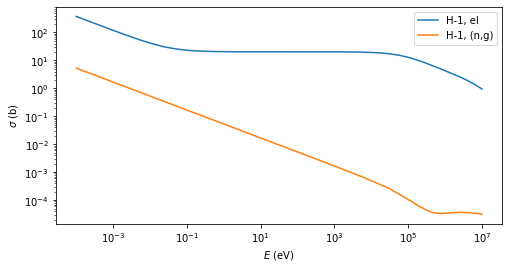
\includegraphics[width=0.82\textwidth]{figures/hw05_h1_cross_sections.png}
\end{center}

The elastic-scattering cross section is nearly constant at about 20~b over a
large part of the low- and intermediate-energy range, and then decreases in
the fast range.  In contrast, the radiative-capture cross section decreases
approximately as $1/v$ over the low-energy range.  Because
$v\propto\sqrt{E}$,
\[
 \sigma_\gamma(E)\propto\frac{1}{v}\propto E^{-1/2}.
\]
Thus, the capture curve is approximately a straight line with slope $-1/2$
on the log--log plot.  The evaluated curve departs from a perfect $1/v$ law
at higher energies.

For reference, the values extracted below are
\[
\begin{array}{c|cc}
 &1~\mathrm{eV}&1~\mathrm{MeV}\\
\hline
\sigma_e&20.5933~\mathrm{b}&4.28306~\mathrm{b}\\
\sigma_\gamma&5.31149\times10^{-2}~\mathrm{b}
              &3.38313\times10^{-5}~\mathrm{b}.
\end{array}
\]

\noindent\emph{Data note:} The plotted curves and quoted values are from the
archived BNL SIGMA/ENDF evaluation used in the Fall 2026 course notebook.  A
fresh export from another evaluated library or processing temperature may
differ slightly.
\end{draftsolution}

\newpage

% --------------------------------------------------------------------------
% Problem 3
% Numerical work follows ne630/notebooks/lesson_05.ipynb, cells 11--12.
% --------------------------------------------------------------------------
\noindent{\bf Problem 3}.  Using \textbf{Evaluated Data} in the Sigma
interface, extract the following cross sections at $1~\mathrm{eV}$ and
$1~\mathrm{MeV}$.  Use linear interpolation as needed.

\begin{center}
\begin{tabular}{|l|c|c|}
\hline
Quantity for \isoA{H}{1}&$1~\mathrm{eV}$&$1~\mathrm{MeV}$\\
\hline
$\sigma_e~(\mathrm{b})$&&\\
$\sigma_\gamma~(\mathrm{b})$&&\\
$\sigma_t~(\mathrm{b})$&&\\
\hline
\end{tabular}
\end{center}

\noindent\emph{Interpolation note:} Given $(x_1,y_1)$ and $(x_2,y_2)$,
evaluate $y$ at $x$, where $x_1<x<x_2$, using
\[
 y(x)=\frac{(x-x_1)y_2+(x_2-x)y_1}{x_2-x_1}.
\]
\textbf{Hint:} Based on the available reactions, do you need to look up
$\sigma_t$, or can you construct it from the partial cross sections?

\begin{draftsolution}
Using the interpolation expression in the problem statement, the
elastic-scattering cross section at 1~eV is
\[
\begin{split}
 \sigma_e(1~\mathrm{eV})
 &=\frac{(1-0.40461)(20.2988)+(1.68858-1)(20.848)}
         {1.68858-0.40461}\\
 &\approx20.5933~\mathrm{b}.
\end{split}
\]
Similarly,
\[
\begin{split}
 \sigma_\gamma(1~\mathrm{eV})
 &=\frac{(1-0.826569)(0.0509196)+(1.07619-1)(0.0581121)}
         {1.07619-0.826569}\\
 &\approx0.0531149~\mathrm{b}.
\end{split}
\]

At 1~MeV, the corresponding interpolations give
\[
\begin{split}
 \sigma_e(1~\mathrm{MeV})
 &=\frac{(10^6-850000)(4.0527)+(1097760-10^6)(4.63652)}
         {1097760-850000}\\
 &\approx4.28306~\mathrm{b},\\[4pt]
 \sigma_\gamma(1~\mathrm{MeV})
 &=\frac{(10^6-800000)(3.67662\times10^{-5})
       +(2000000-10^6)(3.32443\times10^{-5})}
         {2000000-800000}\\
 &\approx3.38313\times10^{-5}~\mathrm{b}.
\end{split}
\]

At these two energies, the available interactions for \isoA{H}{1} are
elastic scattering and radiative capture.  Hence,
\[
 \sigma_t=\sigma_e+\sigma_\gamma.
\]
The completed table is
\begin{center}
\begin{tabular}{|l|r|r|}
\hline
Quantity for \isoA{H}{1}&$1~\mathrm{eV}$&$1~\mathrm{MeV}$\\
\hline
$\sigma_e~(\mathrm{b})$&20.5933&4.28306\\
$\sigma_\gamma~(\mathrm{b})$&0.0531149&$3.38313\times10^{-5}$\\
$\sigma_t~(\mathrm{b})$&20.6464&4.28309\\
\hline
\end{tabular}
\end{center}

\noindent\emph{Data note:} These numbers use the interpolation points stored
in the archived course notebook.  Their last quoted digits are evaluation-
and interpolation-dependent.
\end{draftsolution}

\newpage
% --------------------------------------------------------------------------
% Problem 4
% Figure is the embedded output of ne630/notebooks/lesson_05.ipynb, cell 15.
% --------------------------------------------------------------------------
\noindent{\bf Problem 4}.  Determine which interaction $X$ dominates the
total cross section of \isoA{B}{10}.  How does $\sigma_X(E)$ depend on $E$?

\noindent\textbf{Hint:} Straight lines on log--log plots indicate power laws
of the form $y(x)=x^p$.

\begin{draftsolution}
The available partial cross sections are shown below.

\begin{center}
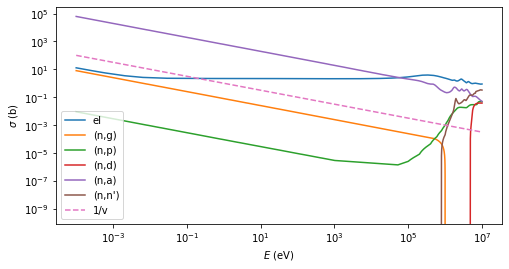
\includegraphics[width=0.82\textwidth]{figures/hw05_b10_cross_sections.png}
\end{center}

The dominant low-energy interaction is
\[
 \isoA{B}{10}(n,\alpha)\isoA{Li}{7}.
\]
Away from the higher-energy structure, the $(n,\alpha)$ cross section is
approximately a $1/v$ cross section:
\[
 \boxed{\sigma_\alpha(E)\propto\frac{1}{v}\propto E^{-1/2}}.
\]
This appears as a straight line with slope $-1/2$ on a log--log plot.

At fast-neutron energies, elastic and inelastic scattering become comparable
to, and eventually larger than, the $(n,\alpha)$ cross section.  Thus,
``dominant'' here refers to the broad low-energy range for which \isoA{B}{10}
is normally used as a neutron absorber; it does not mean that $(n,\alpha)$ is
the largest partial cross section at every energy shown.
\end{draftsolution}

\newpage

% --------------------------------------------------------------------------
% Problem 5
% Values follow ne630/notebooks/lesson_05.ipynb and
% ne630_problems/lesson_05/HW05_solution_work.ipynb.
% --------------------------------------------------------------------------
\noindent{\bf Problem 5}.  Using the Sigma interface, determine the missing
values in the following table.  All cross sections are in barns.

\begin{center}
\begin{tabular}{|l|l|c|c|}
\hline
Nuclide&Quantity&$1~\mathrm{eV}$&$1~\mathrm{MeV}$\\
\hline
\isoA{U}{235}&$\sigma_t$&&\\
\isoA{U}{235}&$\sigma_e$&&\\
\isoA{U}{235}&$\sigma_\gamma$&&\\
\isoA{U}{235}&$\sigma_f$&&\\
\isoA{U}{235}&$\bar\nu$&&\\
\isoA{U}{238}&$\sigma_t$&&\\
\isoA{U}{238}&$\sigma_e$&&\\
\isoA{U}{238}&$\sigma_\gamma$&&\\
\isoA{U}{238}&$\sigma_f$&&\\
\isoA{U}{238}&$\bar\nu$&&\\
\hline
\end{tabular}
\end{center}

\begin{draftsolution}
Here, I'm using the actual text files from BNL Sigma, so these numbers ought
to be the same that you get by hand/calculator.

\begin{center}
\begin{tabular}{|l|l|r|r|}
\hline
Nuclide&Quantity&$1~\mathrm{eV}$&$1~\mathrm{MeV}$\\
\hline
\isoA{U}{235}&$\sigma_t~(\mathrm{b})$&91.60&6.85619\\
\isoA{U}{235}&$\sigma_e~(\mathrm{b})$&13.14&3.65029\\
\isoA{U}{235}&$\sigma_\gamma~(\mathrm{b})$&10.40&0.108433\\
\isoA{U}{235}&$\sigma_f~(\mathrm{b})$&67.77&1.19979\\
\isoA{U}{235}&$\bar\nu$&2.421&2.51601\\
\hline
\isoA{U}{238}&$\sigma_t~(\mathrm{b})$&9.687&7.12538\\
\isoA{U}{238}&$\sigma_e~(\mathrm{b})$&9.085&4.72403\\
\isoA{U}{238}&$\sigma_\gamma~(\mathrm{b})$&0.5105&0.128299\\
\isoA{U}{238}&$\sigma_f~(\mathrm{b})$&$2.963\times10^{-6}$&0.0135521\\
\isoA{U}{238}&$\bar\nu$&2.492&2.56336\\
\hline
\end{tabular}
\end{center}

The small \isoA{U}{238} fission cross section at 1~eV is not a typo.
Fission of \isoA{U}{238} is possible at low energies in the evaluated data,
but it is extremely improbable.  Its fission cross section increases
substantially in the fast range, which is why \isoA{U}{238} is normally
described as a threshold-fission nuclide.

\medskip
\noindent\emph{Data note:} The 1-eV values are retained as rounded constants
in the Fall 2026 course notebook; the raw SIGMA text files are not present in
the repository.  The 1-MeV values are preserved at greater precision in the
archived solution notebook.  These are values from that archived evaluation,
not library-independent constants.
\end{draftsolution}

\newpage

% --------------------------------------------------------------------------
% Problem 6
% Opening/process language follows the style of the original lesson_05
% solution; numerical work follows ne630/notebooks/lesson_05.ipynb,
% cells 19--29. No matching solution exists for the current problem.
% --------------------------------------------------------------------------
\noindent{\bf Problem 6}.  Our TRIGA fuel consists of a mixture of zirconium
hydride ($\mathrm{ZrH}_{1.6}$) and uranium metal with a bulk mass density of
$7.1~\mathrm{g\,cm^{-3}}$.
\begin{itemize}
\item Uranium makes up 8.5\% of the mixture \textbf{by mass}.
\item The uranium is enriched to 20\% \isoA{U}{235} \textbf{by atom}; assume
the balance is \isoA{U}{238}.
\item Natural zirconium consists of \isoA{Zr}{90} (51.5\%), \isoA{Zr}{91}
(11.2\%), \isoA{Zr}{92} (17.1\%), \isoA{Zr}{94} (17.4\%), and \isoA{Zr}{96}
(2.8\%), all by atom.
\item Assume that \isoA{H}{1}, \isoA{U}{235}, and \isoA{U}{238} are the only
other nuclides.
\end{itemize}
Use $N_A=6.022\times10^{23}~\mathrm{mol^{-1}}$ and approximate each isotope's
molar mass by its mass number in $\mathrm{g\,mol^{-1}}$.

\begin{enumerate}[label=(\alph*)]
\item Compute the indicated molecular and atomic number densities.  The
following expressions provide a starting point:
\[
\begin{gathered}
\overline M_{\mathrm{Zr}}
=0.515(90)+0.112(91)+0.171(92)+0.174(94)+0.028(96),\\
M_{\mathrm{ZrH}_{1.6}}=\overline M_{\mathrm{Zr}}+1.6(1),\qquad
n_{\mathrm{ZrH}_{1.6}}
=\frac{(0.915)(7.1)N_A}{M_{\mathrm{ZrH}_{1.6}}},\\
n_{\isoA{H}{1}}=1.6n_{\mathrm{ZrH}_{1.6}},\qquad
n_{\isoA{Zr}{90}}=0.515n_{\mathrm{ZrH}_{1.6}},\\[2pt]
\overline M_{\mathrm U}=0.20(235)+0.80(238),\qquad
n_{\mathrm U}=\frac{(0.085)(7.1)N_A}{\overline M_{\mathrm U}},\\
n_{\isoA{U}{235}}=0.20n_{\mathrm U},\qquad
n_{\isoA{U}{238}}=0.80n_{\mathrm U}.
\end{gathered}
\]
Report all six requested densities: $n_{\mathrm{ZrH}_{1.6}}$,
$n_{\isoA{H}{1}}$, $n_{\isoA{Zr}{90}}$, $n_{\mathrm U}$,
$n_{\isoA{U}{235}}$, and $n_{\isoA{U}{238}}$.
\item Suppose the elastic-scattering cross section for zirconium, averaged
over its naturally occurring isotopes, is $6~\mathrm b$ at all neutron
energies and that all other interactions with zirconium are negligible.
Using the cross sections collected above, compute the macroscopic total,
elastic-scattering, and absorption cross sections of the fuel at $1~\mathrm{eV}$.
\item If a $1~\mathrm{eV}$ neutron interacts in the fuel, what is the
probability that the interaction is an elastic collision?
\item If a $1~\mathrm{eV}$ neutron has an elastic collision, what is the
probability that it collides with \isoA{H}{1}?
\item On average, how far does a $1~\mathrm{eV}$ neutron travel in this fuel
before undergoing any interaction?
\item If a $1~\mathrm{eV}$ neutron is absorbed, what is the probability that
it induces fission?
\item If a $1~\mathrm{eV}$ neutron induces fission, what is the expected
number of emitted neutrons?  Account for both uranium isotopes by using a
fission-rate-weighted value of $\bar\nu$.
\end{enumerate}

\begin{draftsolution}
To answer (a)--(g), we need to compute the number density of each nuclide in
the fuel mixture and to evaluate macroscopic cross sections for each nuclide
and reaction.  Given the tabular data and repeated calculations, it is far
more convenient to use a short script (in, e.g., Python) or a spreadsheet than
to do each calculation by hand.  Here, I'm using Python to do the computations.

\begin{enumerate}[label=(\alph*)]
\item First, I'll compute the number densities given the mass density,
chemical formula, and uranium enrichment.  The average molar mass of natural
zirconium is
\[
\begin{split}
 \overline M_{\mathrm{Zr}}
 &=0.515(90)+0.112(91)+0.171(92)+0.174(94)+0.028(96)\\
 &=91.318~\mathrm{g/mol}.
\end{split}
\]
Therefore,
\[
 M_{\mathrm{ZrH}_{1.6}}=91.318+1.6(1)=92.918~\mathrm{g/mol}.
\]
The zirconium-hydride portion of the fuel has an effective mass density
$(1-0.085)(7.1)=6.4965~\mathrm{g/cm^3}$, and hence
\[
\begin{split}
 n_{\mathrm{ZrH}_{1.6}}
 &=\frac{(0.915)(7.1)(6.022\times10^{23})}{92.918}\\
 &=4.21037\times10^{22}~\mathrm{cm^{-3}}.
\end{split}
\]
There is one zirconium atom and 1.6 hydrogen atoms per formula unit, so
\[
\begin{split}
 n_{\isoA{H}{1}}&=1.6n_{\mathrm{ZrH}_{1.6}}
 =6.73659\times10^{22}~\mathrm{cm^{-3}},\\
 n_{\isoA{Zr}{90}}&=0.515n_{\mathrm{ZrH}_{1.6}}
 =2.16834\times10^{22}~\mathrm{cm^{-3}}.
\end{split}
\]
For the uranium,
\[
 \overline M_{\mathrm U}=0.20(235)+0.80(238)=237.4~\mathrm{g/mol},
\]
so that
\[
\begin{split}
 n_{\mathrm U}
 &=\frac{(0.085)(7.1)(6.022\times10^{23})}{237.4}
 =1.53087\times10^{21}~\mathrm{cm^{-3}},\\
 n_{\isoA{U}{235}}&=0.20n_{\mathrm U}
 =3.06173\times10^{20}~\mathrm{cm^{-3}},\\
 n_{\isoA{U}{238}}&=0.80n_{\mathrm U}
 =1.22469\times10^{21}~\mathrm{cm^{-3}}.
\end{split}
\]
Thus, all six requested densities are
\begin{center}
\begin{tabular}{|l|r|r|}
\hline
Quantity&$\mathrm{cm^{-3}}$&$\mathrm{(b\,cm)^{-1}}$\\
\hline
$n_{\mathrm{ZrH}_{1.6}}$&$4.21037\times10^{22}$&0.0421037\\
$n_{\isoA{H}{1}}$&$6.73659\times10^{22}$&0.0673659\\
$n_{\isoA{Zr}{90}}$&$2.16834\times10^{22}$&0.0216834\\
$n_{\mathrm U}$&$1.53087\times10^{21}$&0.00153087\\
$n_{\isoA{U}{235}}$&$3.06173\times10^{20}$&0.000306173\\
$n_{\isoA{U}{238}}$&$1.22469\times10^{21}$&0.00122469\\
\hline
\end{tabular}
\end{center}
For the individual nuclides, I've adopted the useful unit of a/b-cm.  This
unit builds in the factor of $10^{-24}~\mathrm{cm^2/b}$ so that $\Sigma$'s
can be computed directly.

\item Then, I compute the individual nuclide-reaction, macroscopic cross
sections.  Using the 1-eV values from Problem 5, the hydrogen values from
Problem 3, and $\sigma_e^{\mathrm{Zr}}=6~\mathrm b$ gives
\[
\begin{split}
 \Sigma_e=10^{-24}\big[&n_{\isoA{U}{235}}(13.14)
 +n_{\isoA{U}{238}}(9.085)+n_{\mathrm{ZrH}_{1.6}}(6)\\
 &+n_{\isoA{H}{1}}(20.5933)\big]
 \approx\boxed{1.65506~\mathrm{cm^{-1}}},
\end{split}
\]
and
\[
\begin{split}
 \Sigma_a=10^{-24}\big[&n_{\isoA{U}{235}}(10.40+67.77)
 +n_{\isoA{U}{238}}(0.5105+2.963\times10^{-6})\\
 &+n_{\isoA{H}{1}}(0.0531149)\big]
 \approx\boxed{0.0281369~\mathrm{cm^{-1}}}.
\end{split}
\]
Using the tabulated total cross sections,
\[
\begin{split}
 \Sigma_t=10^{-24}\big[&n_{\isoA{U}{235}}(91.60)
 +n_{\isoA{U}{238}}(9.687)+n_{\mathrm{ZrH}_{1.6}}(6)\\
 &+n_{\isoA{H}{1}}(20.6464)\big]
 \approx\boxed{1.68340~\mathrm{cm^{-1}}}.
\end{split}
\]
The small difference between $\Sigma_t$ and $\Sigma_e+\Sigma_a$ is due to
the precision retained in the archived, separately interpolated microscopic
cross sections and any small channels not listed individually.

\item If a neutron interacts, the probability that the interaction is an
elastic collision is
\[
 P(e\mid t)=\frac{R_e}{R_t}=\frac{\Sigma_e\phi}{\Sigma_t\phi}
 =\frac{\Sigma_e}{\Sigma_t}
 =\frac{1.65506}{1.68340}\approx\boxed{0.9832}.
\]

\item The macroscopic elastic-scattering cross section of hydrogen alone is
\[
 \Sigma_e^{\isoA{H}{1}}=n_{\isoA{H}{1}}\sigma_e^{\isoA{H}{1}}
 \approx1.38729~\mathrm{cm^{-1}}.
\]
Therefore, given that an elastic collision occurred,
\[
 P(\isoA{H}{1}\mid e)=\frac{\Sigma_e^{\isoA{H}{1}}}{\Sigma_e}
 =\frac{1.38729}{1.65506}\approx\boxed{0.8382}.
\]

\item The average distance to any interaction is the mean free path:
\[
 \lambda=\frac{1}{\Sigma_t}=\frac{1}{1.68340}
 \approx\boxed{0.5940~\mathrm{cm}}.
\]

\item The macroscopic fission cross section is
\[
\begin{split}
 \Sigma_f=10^{-24}\big[n_{\isoA{U}{235}}(67.77)
 +n_{\isoA{U}{238}}(2.963\times10^{-6})\big]
 =0.0207494~\mathrm{cm^{-1}}.
\end{split}
\]
Consequently, given that an absorption occurred,
\[
 P(f\mid a)=\frac{\Sigma_f}{\Sigma_a}
 =\frac{0.0207494}{0.0281369}\approx\boxed{0.7374}.
\]

\item Finally, the fission-rate-weighted neutron yield is
\[
 \overline\nu=
 \frac{\overline\nu_{\isoA{U}{235}}\Sigma_f^{\isoA{U}{235}}
       +\overline\nu_{\isoA{U}{238}}\Sigma_f^{\isoA{U}{238}}}
      {\Sigma_f^{\isoA{U}{235}}+\Sigma_f^{\isoA{U}{238}}}.
\]
Using
\[
 \Sigma_f^{\isoA{U}{235}}=0.020749364~\mathrm{cm^{-1}},\qquad
 \Sigma_f^{\isoA{U}{238}}=3.62877\times10^{-9}~\mathrm{cm^{-1}},
\]
and $\overline\nu_{\isoA{U}{235}}=2.421$ and
$\overline\nu_{\isoA{U}{238}}=2.492$ gives
\[
 \boxed{\overline\nu\approx2.421\text{ neutrons per fission}}.
\]
The \isoA{U}{238} contribution is negligible at 1~eV, so the result is
effectively the \isoA{U}{235} value.
\end{enumerate}

\noindent\emph{Data note:} Parts (b)--(g) inherit the rounded, archived BNL
SIGMA/ENDF values used in Problems 3 and 5.  The displayed arithmetic is
internally consistent with those values, but the extra digits should not be
interpreted as physical accuracy.
\end{draftsolution}

\clearpage


\HomeworkSection{Homework 06: Lesson 06}
% Assignment source: ne630/homework/markdown/HW06.md.
% Legacy foundation: ne630_problems/lesson_06/statement.tex @ e1fba66.
% Problem 1 is new for Fall 2026. Problem 2 adapts legacy Problem 1, and
% Problem 3 adapts legacy Problem 2 to determine the normalization explicitly.

% --------------------------------------------------------------------------
% Problem 1
% --------------------------------------------------------------------------
\noindent{\bf Problem 1}. Use OpenMC's Python nuclear-data interface to
examine the radiative-capture cross section, $\sigma_\gamma(E)$, of
\isoA{U}{238}. No transport calculation is required. On Beocat, the
continuous-energy data file is
\begin{center}
\texttt{/homes/jaroberts/openmc/data/neutron/U238.h5}.
\end{center}
Load this file with \texttt{openmc.data.IncidentNeutron.from\_hdf5}, use the
radiative-capture reaction (ENDF MT 102), and select the \texttt{"294K"}
cross section. The resulting callable takes neutron energy in eV and returns
the microscopic cross section in barns.

\begin{enumerate}[label=(\alph*)]
\item Plot $\sigma_\gamma(E)$ over $10^{-4}\leq E\leq10^7~\mathrm{eV}$
using log--log axes.
\item Above approximately what energy do the individual resonance peaks begin
to overlap and appear as a relatively smooth curve?
\item Plot $\sigma_\gamma(E)$ again over $1\leq E\leq100~\mathrm{eV}$ using
a linear energy axis and a logarithmic cross-section axis.
\item At what energy is the first large resonance peak?
\end{enumerate}
Use energy meshes fine enough to resolve the narrow resonances. Increase the
mesh resolution until the plotted resonance locations and heights no longer
change visibly.

\begin{draftsolution}
I loaded the 294~K, MT-102 cross section directly from the OpenMC HDF5 file.
For example, the data and two plotting meshes can be prepared with
\begin{minted}{python}
import numpy as np
import openmc

data_path = "/homes/jaroberts/openmc/data/neutron/U238.h5"
u238 = openmc.data.IncidentNeutron.from_hdf5(data_path)
sigma_gamma = u238.reactions[102].xs["294K"]

E_full = np.geomspace(1.0e-4, 1.0e7, 500_000)
E_resolved = np.linspace(1.0, 100.0, 1_000_001)
sig_full = sigma_gamma(E_full)
sig_resolved = sigma_gamma(E_resolved)
\end{minted}
The wide-range result is
\begin{center}
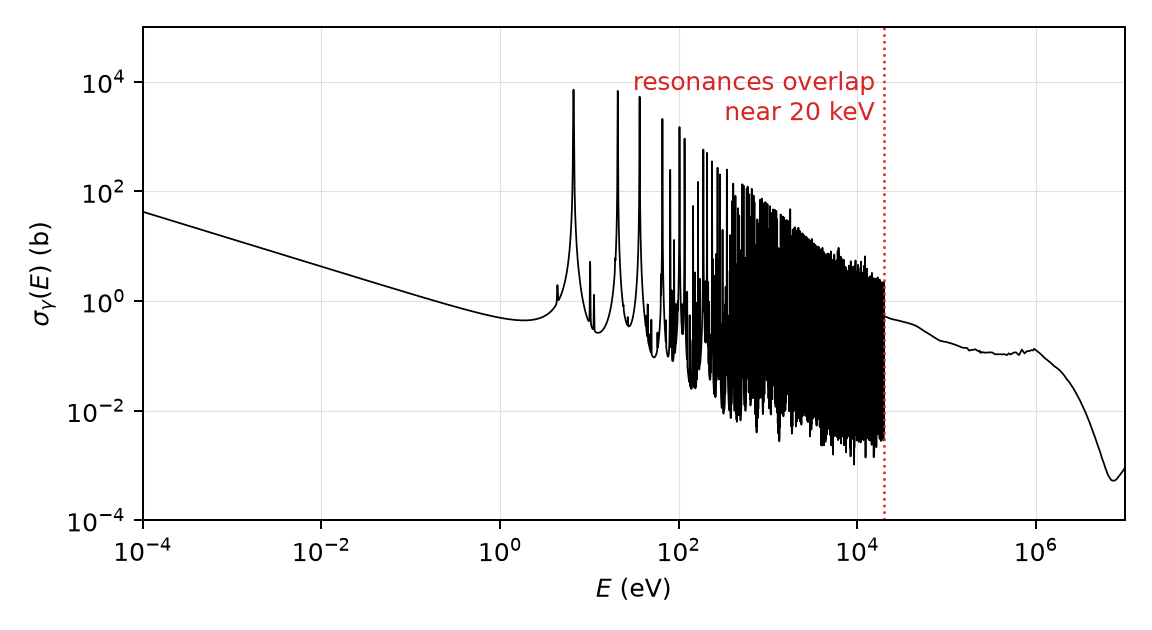
\includegraphics[width=0.86\textwidth]{figures/hw06_u238_capture_full.png}
\end{center}
At low energy, the resonances are well separated. At about
$\boxed{2\times10^4~\mathrm{eV}}$, or $20~\mathrm{keV}$, they begin to
overlap and the evaluated cross section appears relatively smooth on this
scale.

Restricting the energy interval gives
\begin{center}
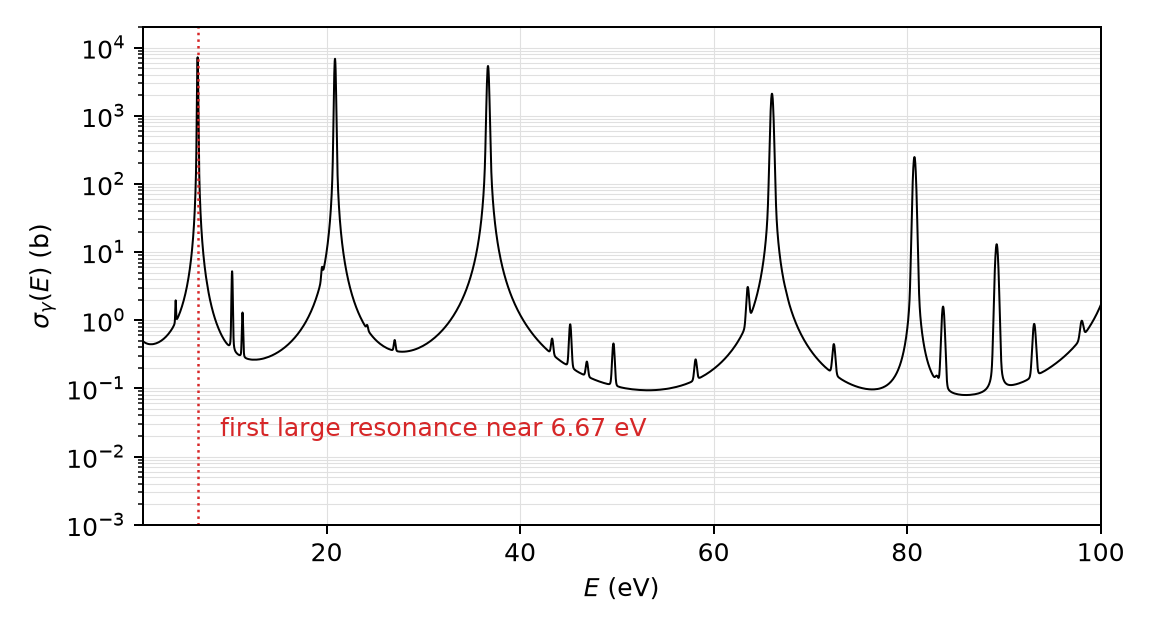
\includegraphics[width=0.86\textwidth]{figures/hw06_u238_capture_1_100ev.png}
\end{center}
The first large resonance is at approximately
$\boxed{E_r=6.67~\mathrm{eV}}$. On the native 294~K tabulation used for the
figure, the local maximum occurs at $6.67428~\mathrm{eV}$; the extra digits
describe the processed energy grid rather than the accuracy with which the
resonance energy should be reported.

I repeated the $1$--$100~\mathrm{eV}$ plot with successively finer uniform
meshes down to $\Delta E\simeq10^{-4}~\mathrm{eV}$. The visible peak
locations and heights no longer changed at the plotting resolution. Using
the native tabulation gives the same plotted result and avoids skipping any
of the energy knots stored in the HDF5 file.
\end{draftsolution}

\newpage

% --------------------------------------------------------------------------
% Problem 2
% The fifth neutron width is 1.874e-3 eV in the Fall 2026 assignment. The
% archived lesson06_sol.ipynb used 1.874e-2 eV; that factor-of-ten typo is not
% propagated here.
% --------------------------------------------------------------------------
\noindent{\bf Problem 2}. Reconstruct the \isoA{U}{238} radiative-capture
cross section over $1\leq E\leq100~\mathrm{eV}$ with the single-level
Breit--Wigner (SLBW) approximation. For resonance $i$,
\[
 \Gamma_i=\Gamma_{n,i}+\Gamma_{\gamma,i},
 \qquad
 \lambda_i=\frac{4.55\times10^{-10}~\mathrm{cm}}
 {\sqrt{E_{r,i}/(1~\mathrm{eV})}},
\]
\[
 \sigma_{0,i}=4\pi\lambda_i^2\frac{\Gamma_{n,i}}{\Gamma_i},
\]
\[
 \sigma_{\gamma,i}(E)
 =\sigma_{0,i}\frac{\Gamma_{\gamma,i}}{\Gamma_i}
 \left(\frac{E_{r,i}}{E}\right)^{1/2}
 \frac{1}{1+4(E-E_{r,i})^2/\Gamma_i^2},
\]
and
\[
 \sigma_\gamma^{\mathrm{SLBW}}(E)=\sum_i\sigma_{\gamma,i}(E).
\]
All energies and widths in these expressions are in eV. The expression for
$\sigma_{0,i}$ produces an area in $\mathrm{cm^2}$; use
$1~\mathrm{b}=10^{-24}~\mathrm{cm^2}$ to report cross sections in barns.
Treat the SLBW reconstruction as a $0~\mathrm{K}$ result.

\begin{center}
\begin{tabular}{rcc}
\toprule
$E_{r,i}$ (eV)&$\Gamma_{n,i}$ (eV)&$\Gamma_{\gamma,i}$ (eV)\\
\midrule
6.67   &$1.476\times10^{-3}$&$2.300\times10^{-2}$\\
20.87  &$1.009\times10^{-2}$&$2.286\times10^{-2}$\\
36.68  &$3.355\times10^{-2}$&$2.300\times10^{-2}$\\
66.03  &$2.418\times10^{-2}$&$2.331\times10^{-2}$\\
80.75  &$1.874\times10^{-3}$&$2.339\times10^{-2}$\\
102.56 &$7.077\times10^{-2}$&$2.408\times10^{-2}$\\
\bottomrule
\end{tabular}
\end{center}
Although the last resonance is centered just above the plotted interval,
include its contribution to the sum.

\begin{enumerate}[label=(\alph*)]
\item Compute and plot $\sigma_\gamma^{\mathrm{SLBW}}(E)$ over
$1\leq E\leq100~\mathrm{eV}$ using a linear energy axis and a logarithmic
cross-section axis.
\item On the same axes, plot the $294~\mathrm{K}$ OpenMC cross section from
Problem 1(c).
\item Compare the two curves. Discuss the resonance locations, peak heights,
peak widths, and any structure not reproduced by the six-resonance SLBW
model. Explain the principal physical reason for the difference in peak
height and width between the $0~\mathrm{K}$ SLBW result and the
$294~\mathrm{K}$ OpenMC data.
\end{enumerate}
Use a sufficiently fine linear energy grid or local refinement near each
resonance, and demonstrate that the reconstructed peaks are converged with
respect to the grid resolution.

\begin{adaptedsolution}
The cross-section values reconstructed from the SLBW approximation are shown
below with values taken from OpenMC. As in the in-class demo, I've used
Python, but Excel or other tools are perfectly acceptable.
\begin{minted}{python}
Er = np.array([6.67, 20.87, 36.68, 66.03, 80.75, 102.56])
Gn = np.array([1.476e-3, 1.009e-2, 3.355e-2,
               2.418e-2, 1.874e-3, 7.077e-2])
Gg = np.array([2.300e-2, 2.286e-2, 2.300e-2,
               2.331e-2, 2.339e-2, 2.408e-2])

E = np.linspace(1.0, 100.0, 1_980_001)  # Delta E = 5e-5 eV
sigma_slbw = np.zeros_like(E)
for Er_i, Gn_i, Gg_i in zip(Er, Gn, Gg):
    Gamma_i = Gn_i + Gg_i
    lambda_i = 4.55e-10/np.sqrt(Er_i)
    sigma_0_i = 4*np.pi*lambda_i**2*Gn_i/Gamma_i
    sigma_slbw += (1.0e24*sigma_0_i*(Gg_i/Gamma_i)
                   * np.sqrt(Er_i/E)
                   / (1.0 + 4.0*(E-Er_i)**2/Gamma_i**2))
\end{minted}

\begin{center}
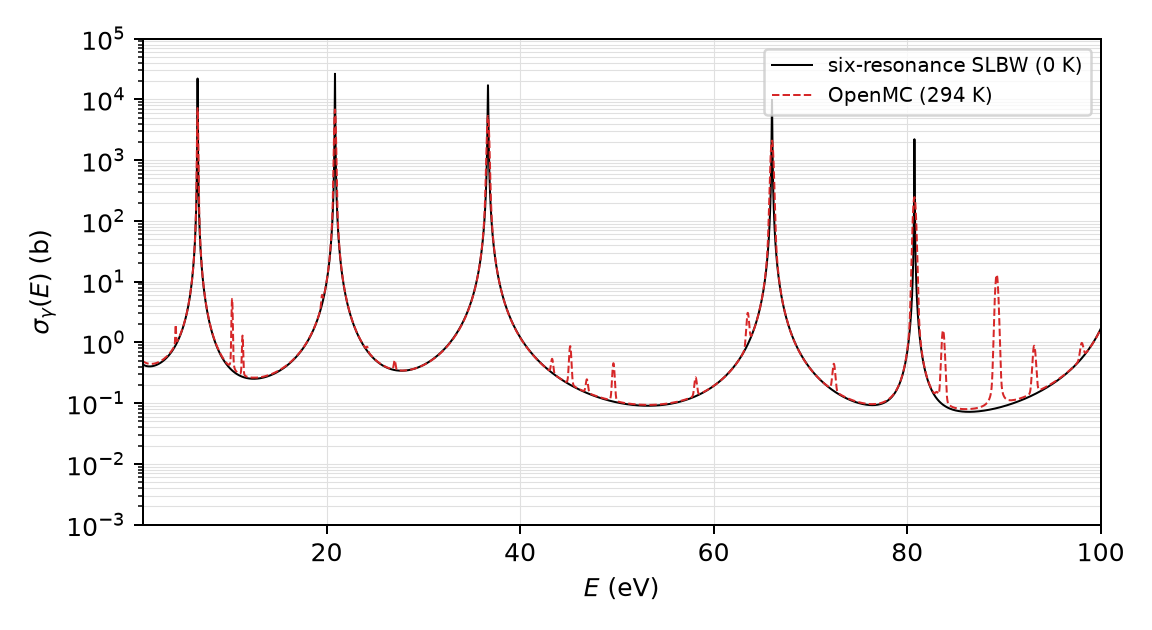
\includegraphics[width=0.88\textwidth]{figures/hw06_slbw_comparison.png}
\end{center}

Overall, the SLBW values are quite close in resonance location for the five
principal resonances exhibited in the energy range. Representative peak and
width values are
\begin{center}\small
\begin{tabular}{rrrr}
\toprule
$E_r$ (eV)&$\Gamma$ (eV)&SLBW peak (b)&294~K OpenMC peak (b)\\
\midrule
6.67  &0.024476&22103&7196\\
20.87 &0.032950&26483&6838\\
36.68 &0.056550&17114&5358\\
66.03 &0.047490& 9847&2101\\
80.75 &0.025264& 2213& 247\\
\bottomrule
\end{tabular}
\end{center}
For an isolated SLBW resonance, the full width at half maximum is
approximately $\Gamma$. The corresponding widths read from the 294~K curve
are about $0.103$, $0.176$, $0.240$, $0.306$, and $0.323~\mathrm{eV}$,
respectively. Thus, the SLBW values exhibit narrower and taller resonances
than the OpenMC data.

The six-resonance sum is also missing fine detail and background structure
that cannot be captured by this model. Recall from class that the OpenMC data
are provided at 294~K. On the other hand, the SLBW model here provides values
for 0~K. The increased temperature leads to \emph{Doppler broadening}, which
spreads each resonance over a wider energy interval and lowers its peak while
approximately preserving its resonance area. The 102.56-eV resonance must be
included even though its center lies outside the plot: at $100~\mathrm{eV}$,
its tail contributes $1.669~\mathrm b$ of the $1.677~\mathrm b$ SLBW total.

I reduced the uniform SLBW grid spacing from $10^{-3}$ to
$5\times10^{-5}~\mathrm{eV}$. The resonance locations and quoted peak
heights were unchanged at the shown precision, and the plotted curves were
visually indistinguishable. The final grid places about 490 points across
even the narrowest total resonance width.
\end{adaptedsolution}

\newpage

% --------------------------------------------------------------------------
% Problem 3
% Numerical values reproduce the legacy approach but normalize the spectrum
% before evaluating either requested probability.
% --------------------------------------------------------------------------
\noindent{\bf Problem 3 [adapted from FNRP 2.9]}. The fission-neutron energy
spectrum is modeled by
\[
 \chi(E)=C\exp(-1.036E)\sinh\!\left(\sqrt{2.29E}\right),
 \qquad E\geq0,
\]
where $E$ is in MeV, $\chi(E)$ is a probability density per MeV, and $C$ is
an unknown normalization constant. Use numerical integration and the
normalized form of $\chi(E)$ to determine the following. Report $C$ and each
fraction to at least three significant figures.

\begin{enumerate}[label=(\alph*)]
\item Evaluate the required integral over the whole domain,
$0\leq E<\infty$, and determine $C$ such that
\[
 \int_0^\infty\chi(E)\,dE=1.
\]
\item Evaluate the fraction of fission neutrons born with energies in
$0\leq E\leq0.1~\mathrm{MeV}$.
\item Evaluate the fraction of fission neutrons born with energies in
$10~\mathrm{MeV}\leq E<\infty$.
\end{enumerate}
Integrate over each stated interval directly. If the numerical method
replaces $\infty$ with a finite upper limit, demonstrate that the result has
converged as that limit is increased.

\begin{adaptedsolution}
The distribution of fission-neutron energies is modeled by
\[
 \chi(E)=C\exp(-1.036E)\sinh(\sqrt{2.29E}),
\]
where $E$ is in MeV. This is definitely a problem best solved using a
numerical technique. Here, I'm using \texttt{scipy.integrate.quad}:
\begin{minted}{python}
import numpy as np
from scipy.integrate import quad

g = lambda E: np.exp(-1.036*E)*np.sinh(np.sqrt(2.29*E))
I = quad(g, 0.0, np.inf)[0]
C = 1.0/I
chi = lambda E: C*g(E)

p_below = quad(chi, 0.0, 0.1)[0]
p_above = quad(chi, 10.0, np.inf)[0]
\end{minted}

\begin{enumerate}[label=(\alph*)]
\item The unnormalized integral is
\[
 I=\int_0^\infty
 \exp(-1.036E)\sinh(\sqrt{2.29E})\,dE
 \approx2.210125128.
\]
Therefore,
\[
 \boxed{C=\frac{1}{I}\approx0.452463070~\mathrm{MeV^{-1}}}.
\]

\item Direct integration over the requested interval gives
\[
 \int_0^{0.1}\chi(E)\,dE
 \approx\boxed{0.0138794},
\]
or about $1.39\%$ of the fission neutrons.

\item Direct integration over the high-energy tail gives
\[
 \int_{10}^{\infty}\chi(E)\,dE
 \approx\boxed{0.00106030},
\]
or about $0.106\%$ of the fission neutrons.
\end{enumerate}

As a finite-upper-limit check, using upper limits of 20, 30, and 40~MeV for
the high-energy-tail integral gives $0.00106008$, $0.00106030295$, and
$0.00106030298$, respectively. Likewise, the normalized integral over
$0\leq E\leq40~\mathrm{MeV}$ is $0.99999999999996$. The reported values are
therefore converged well beyond the requested three significant figures.
\end{adaptedsolution}

\clearpage


\HomeworkSection{Homework 07: Lesson 07}
% Assignment source: ne630/homework/html/HW07.html.
% Legacy foundation: ne630_problems/lesson_07/statement.tex @ e1fba66.
% Problem 1 retains the legacy solution while updating part (e) to the OpenMC
% 294 K values requested in Fall 2026. The missing square in the legacy
% definition of alpha is corrected; the worked examples already used it.

% --------------------------------------------------------------------------
% Problem 1
% --------------------------------------------------------------------------
\noindent{\bf Problem 1}. Neutrons scatter elastically at $1.0~\mathrm{MeV}$.
After one scattering collision, determine the fraction of the neutrons that
will have energies less than $0.5~\mathrm{MeV}$ if they scatter from each of
the following:
\begin{enumerate}[label=(\alph*)]
\item Hydrogen
\item Deuterium
\item Carbon-12
\item Uranium-238
\item Light water
\end{enumerate}
For part (e), obtain the H-1 and O-16 elastic-scattering cross sections at
$1.0~\mathrm{MeV}$ using OpenMC's Python nuclear-data interface
(\texttt{openmc.data.IncidentNeutron}). Use the elastic-scattering reaction
(ENDF MT 2) and the \texttt{"294K"} cross section.

\begin{adaptedsolution}
The probability that a neutron of energy $E$ will scatter down to an energy
between $E'$ and $E'+dE'$ after colliding with a target nucleus of mass number
$A$ is given by
\[
 p(E\to E')\,dE'=
 \begin{cases}
 \dfrac{1}{(1-\alpha)E}\,dE',&\alpha E\leq E'\leq E,\\
 0,&\text{otherwise},
 \end{cases}
 \tag{FNRP 2.47}
\]
where
\[
 \alpha=\left(\frac{A-1}{A+1}\right)^2.
\]
Then, the probability that a neutron of energy $E$ scatters to an energy
equal to or less than $E_0$ is
\[
 P(E'\leq E_0)=
 \begin{cases}
 \displaystyle\int_{\alpha E}^{E_0}
 \frac{1}{(1-\alpha)E}\,dE'
 =\dfrac{E_0-\alpha E}{(1-\alpha)E},&E_0>\alpha E,\\[3pt]
 0,&\text{otherwise}.
 \end{cases}
\]
Thus, for $E=1~\mathrm{MeV}$ and $E_0=0.5~\mathrm{MeV}$, we have for each
target nucleus
\begin{enumerate}[label=(\alph*)]
\item $\alpha_{\mathrm H}=(1-1)^2/(1+1)^2=0$, and
\[
 \boxed{P(E'\leq0.5~\mathrm{MeV})=\frac{0.5}{1}=0.5}.
\]

\item $\alpha_{\mathrm D}=(2-1)^2/(2+1)^2=1/9$, and
\[
 \boxed{P(E'\leq0.5~\mathrm{MeV})
 =\frac{0.5-(1/9)1}{(1-1/9)1}=0.4375}.
\]

\item $\alpha_{\mathrm C}=(12-1)^2/(12+1)^2\approx0.716$ and, hence,
$0.5=E_0<\alpha_{\mathrm C}E=0.716$, so
\[
 \boxed{P(E'\leq0.5~\mathrm{MeV})=0}.
\]

\item $\alpha_{\mathrm U}=(238-1)^2/(238+1)^2\approx0.983$, so again
\[
 \boxed{P(E'\leq0.5~\mathrm{MeV})=0}.
\]
\end{enumerate}

For (e), we have a mixture of two nuclides and, hence, we need
\[
 p(E\to E')=\frac{1}{\Sigma_s(E)}
 \sum_i\Sigma_{s i}(E)p_i(E\to E').
 \tag{FNRP 2.53}
\]
For $1~\mathrm{MeV}$ neutrons, the 294~K OpenMC elastic-scattering cross
sections are
\[
 \sigma_s^{\isoA{H}{1}}=4.249507~\mathrm b,
 \qquad
 \sigma_s^{\isoA{O}{16}}=8.125790~\mathrm b.
\]
Because $\alpha_{\isoA{O}{16}}=(15/17)^2\approx0.779$, a $1~\mathrm{MeV}$
neutron cannot scatter off \isoA{O}{16} to energies below
$0.5~\mathrm{MeV}$. We already found that half of $1~\mathrm{MeV}$ neutrons
scatter off \isoA{H}{1} to energies below $0.5~\mathrm{MeV}$. Hence, we just
need
\[
 \frac{\Sigma_s^{\isoA{H}{1}}}{\Sigma_s^{\text{water}}}
 =\frac{2n_w\sigma_s^{\isoA{H}{1}}}
 {2n_w\sigma_s^{\isoA{H}{1}}+n_w\sigma_s^{\isoA{O}{16}}}
 =\frac{2(4.249507)}{2(4.249507)+8.125790}
 \approx0.511225,
\]
where $n_w$ is the number density of water molecules. Therefore,
\[
 \boxed{P(E'\leq0.5~\mathrm{MeV})
 =0.511225(0.5)\approx0.255612}.
\]
\end{adaptedsolution}

\newpage

% --------------------------------------------------------------------------
% Problem 2: solution language retained from the legacy source. One omitted
% line of algebra is displayed explicitly in place of the source's ellipsis.
% --------------------------------------------------------------------------
\noindent{\bf Problem 2}. Show that, for elastic scattering,
\[
 \overline{E-E'}\equiv
 \int_0^E(E-E')p(E\to E')\,dE'
 =\frac{(1-\alpha)E}{2}.
\]

\vspace{0.5cm}
\ifsolved
{
\color{purple}

\noindent{\bf SOLUTION}:

Given a probability density function $p(x)$, recall that the expected value
of some function $f(x)$ is given by $\bar{f}=\int f(x)p(x)\,dx$, where the
integral is over the domain of $x$. Here, our density is $p(E\to E')$, which
can also be written as $p(E';E)$ (i.e., the probability for $E'$ given $E$ as
a known parameter). Then, with $f(E')=E-E'$, we have
\begin{align*}
 \overline{E-E'}
 &=\int_0^E(E-E')p(E\to E')\,dE'\\
 &=\int_{\alpha E}^E(E-E')\frac{1}{(1-\alpha)E}\,dE'\\
 &=\left[\frac{E'}{1-\alpha}
 -\frac{E'^2}{2(1-\alpha)E}\right]_{\alpha E}^E\\
 &=\frac{E}{1-\alpha}
 \left(\frac12-\alpha+\frac{\alpha^2}{2}\right)\\
 &=\boxed{\frac{(1-\alpha)E}{2}}.
\end{align*}

}
\else
% NOTHING
\fi

\clearpage


\HomeworkSection{Homework 08: Lesson 08}
% Assignment source: ne630/homework/html/HW08.html.
% Legacy foundation: ne630_problems/lesson_08/statement.tex and
% ne630_problems/lesson_08/HW08_solution.ipynb.
% Problem 2 keeps the legacy notebook's computed eta values and adds the
% Fall 2026 interpretation prompt.

\noindent{\bf Problem 1}. Following the lecture example, use data from OpenMC
to reproduce Figure 3.2 from FNRP, and add a curve for U enriched to 4\%.
This figure should be produced using computer software (e.g., Python, Excel,
MATLAB) and {\it not} by hand.

\begin{adaptedsolution}
A correct solution computes
\[
 \eta(E)=
 \frac{e\,\bar{\nu}_{235}(E)\sigma_{f,235}(E)
       +(1-e)\,\bar{\nu}_{238}(E)\sigma_{f,238}(E)}
      {e\,\sigma_{a,235}(E)+(1-e)\,\sigma_{a,238}(E)}
\]
for the requested enrichments, where $e$ is the atom fraction of
\isoA{U}{235}.  The absorption cross sections should include capture plus
fission:
\[
 \sigma_a(E)=\sigma_\gamma(E)+\sigma_f(E).
\]

The plotted curves should reproduce the main behavior of FNRP Fig.~3.2: the
natural-uranium curve remains below the enriched cases over most energies, the
20\% curve is highest, and the 4\% curve lies between them.  The raw evaluated
data are noisy where the pointwise cross sections and $\bar{\nu}$ are tabulated
on different energy grids, so interpolation to a common grid is expected.
Smoothing the plotted curve is acceptable for visual comparison, but grading
should be based on the unsmoothed values used in any numerical follow-up.
\end{adaptedsolution}

\newpage

\noindent{\bf Problem 2}. For the 4\% values, compute the expected value of
$\eta(E)$ using
\[
p(E)=
  \begin{cases}
    C, & E_{\mathrm{min}}\le E\le E_{\mathrm{max}},\\
    0, & \text{otherwise},
  \end{cases}
\]
for the following three cases:
\begin{enumerate}[label=(\alph*)]
\item $E_{\mathrm{min}}=10^{-3}~\mathrm{eV}$ and
      $E_{\mathrm{max}}=1~\mathrm{eV}$ (the ``thermal'' range).
\item $E_{\mathrm{min}}=1~\mathrm{eV}$ and
      $E_{\mathrm{max}}=10^5~\mathrm{eV}$ (the ``epithermal'' range).
\item $E_{\mathrm{min}}=10^5~\mathrm{eV}$ and
      $E_{\mathrm{max}}=10^7~\mathrm{eV}$ (the ``fast'' range).
\end{enumerate}
For each case, define $C$ using the properties of probability density
functions; that is,
\[
 \int_{E_{\mathrm{min}}}^{E_{\mathrm{max}}}p(E)\,dE=1.
\]
Generally, reactors are classified as being either ``thermal'' or ``fast''
spectrum reactors. Based on your values for $\bar{\eta}$ in each energy range,
explain why we do not often consider ``intermediate'' spectrum reactors.

\begin{adaptedsolution}
For a uniform probability density over the interval
$[E_{\min},E_{\max}]$,
\[
 C=\frac{1}{E_{\max}-E_{\min}},
 \qquad
 \bar{\eta}
 =\frac{1}{E_{\max}-E_{\min}}
  \int_{E_{\min}}^{E_{\max}}\eta(E)\,dE.
\]
Numerically, the legacy solution notebook evaluates $\eta(E)$ from pointwise
BNL/OpenMC-style data and integrates with the trapezoid rule.  For the full
range $10^{-3}\le E\le10^7~\mathrm{eV}$, the same calculation gives
\[
 \bar{\eta}_{\mathrm{uniform}}\approx 2.82.
\]
If instead the flux-weighting density is taken proportional to $1/E$ over
the full range, the notebook gives
\[
 \bar{\eta}_{1/E}
 =\frac{\int \eta(E)E^{-1}\,dE}{\int E^{-1}\,dE}
 \approx 1.36.
\]

Using the local ENDF/B-VIII.1 OpenMC HDF5 data and a converged logarithmic
energy grid, the three assigned uniform-range averages are approximately
\[
\begin{array}{ll}
10^{-3}\le E\le1~\mathrm{eV}: & \bar{\eta}\approx1.82,\\
1\le E\le10^5~\mathrm{eV}: & \bar{\eta}\approx0.552,\\
10^5\le E\le10^7~\mathrm{eV}: & \bar{\eta}\approx2.85.
\end{array}
\]
The epithermal/intermediate range is dominated by strong resonance absorption
structure and gives a much lower average reproduction factor than either the
thermal or fast range in this calculation.  That is the main physical reason
reactor spectra are usually pushed toward thermal or fast designs rather than
left in an intermediate spectrum.
\end{adaptedsolution}

\newpage

\noindent{\bf Problem 3}. The slowing-down properties of three common
moderators are provided in Table 3.1 of FNRP. Add a row to that table for Be,
another element with small mass, and compare Be as a moderator with
$\mathrm{H}_2\mathrm{O}$, $\mathrm{D}_2\mathrm{O}$, and graphite. You may use
data from Appendix E, Table E.3.

\begin{adaptedsolution}
Natural Be consists only of \isoA{Be}{9} and, from Table~E.3, has a mass
density of $\rho=1.85~\gram\per\centi\meter\cubed$.  Thus
\[
 \alpha=\left(\frac{A-1}{A+1}\right)^2
       =\left(\frac{8}{10}\right)^2=0.64,
\]
and
\[
 \boxed{\xi
 =1+\frac{\alpha}{1-\alpha}\ln\alpha
 \approx0.207}.
\]
The number density of natural Be is
\[
 n_{\mathrm{Be}}
 =\frac{1.85(6.022\times10^{23})}{9.013}
 \approx1.24\times10^{23}~\mathrm{atoms/cm^3}.
\]
Using $\sigma_s=6.151~\mathrm b$ and $\sigma_a=0.0085~\mathrm b$,
\[
 \Sigma_s\approx0.76~\centi\meter^{-1},
 \qquad
 \Sigma_a\approx1.1\times10^{-3}~\centi\meter^{-1}.
\]
Therefore,
\[
 \boxed{\xi\Sigma_s\approx0.157~\centi\meter^{-1}},
 \qquad
 \boxed{\frac{\xi\Sigma_s}{\Sigma_a}\approx1.5\times10^2}.
\]
Be has a slowing-down decrement and slowing-down power between heavy water and
graphite, as expected from its mass.  Its slowing-down ratio is better than
light water but below graphite.  It is plausible as a reflector or specialty
moderating material, but graphite and heavy water remain the more familiar
natural-uranium moderator choices.
\end{adaptedsolution}

\clearpage


\HomeworkSection{Homework 09: Lesson 09}
% Assignment source: ne630/homework/html/HW09.html.
% Legacy foundation: ne630_problems/lesson_09/statement.tex.

\noindent{\bf Problem 1}. Verify Eqs.~(3.23) and (3.25):
\[
 \Sigma_s(E)\varphi(E)=\frac{C}{E}
 \tag{FNRP 3.23}
\]
and
\[
 q=\left[1+\frac{\alpha}{1-\alpha}\ln\alpha\right]C.
 \tag{FNRP 3.25}
\]
\textbf{Hint:} To verify Eq.~(3.23), substitute Eq.~(3.23) into Eq.~(3.22)
and show that the left- and right-hand sides are equal.

\begin{adaptedsolution}
Substitute $\Sigma_s(E)\phi(E)=C/E$ into Eq.~(3.22):
\begin{align*}
 \Sigma_s(E)\phi(E)
 &=\int_E^{E/\alpha}
   \frac{1}{(1-\alpha)E'}\Sigma_s(E')\phi(E')\,dE'\\
 &=\int_E^{E/\alpha}\frac{1}{(1-\alpha)E'}\frac{C}{E'}\,dE'\\
 &=\frac{C}{1-\alpha}\int_E^{E/\alpha}\frac{dE'}{E'^2}\\
 &=\frac{C}{1-\alpha}\left[-\frac{1}{E'}\right]_E^{E/\alpha}\\
 &=\frac{C}{1-\alpha}\left(\frac{1}{E}-\frac{\alpha}{E}\right)
  =\boxed{\frac{C}{E}}.
\end{align*}
For Eq.~(3.25),
\begin{align*}
 q
 &=\int_E^{E/\alpha}
   \left[\int_{\alpha E'}^E
   \frac{1}{(1-\alpha)E'}\Sigma_s(E')\phi(E')\,dE''\right]dE'\\
 &=\frac{C}{1-\alpha}\int_E^{E/\alpha}
   \frac{E-\alpha E'}{E'^2}\,dE'\\
 &=\frac{C}{1-\alpha}
   \left(\int_E^{E/\alpha}\frac{E}{E'^2}\,dE'
         -\int_E^{E/\alpha}\frac{\alpha}{E'}\,dE'\right)\\
 &=\frac{C}{1-\alpha}\left(1-\alpha+\alpha\ln\alpha\right)\\
 &=\boxed{\left[1+\frac{\alpha}{1-\alpha}\ln\alpha\right]C}.
\end{align*}
\end{adaptedsolution}

\newpage

\noindent{\bf Problem 2}. For thermal neutrons, calculate $\bar{\eta}$ as a
function of uranium enrichment and plot your results for enrichments between
0\% and 30\%. Use the uranium data from the following table:
\[
\begin{array}{lrrr}
\toprule
 & \nu & \sigma_f~(\mathrm{barns}) & \sigma_a~(\mathrm{barns})\\
\midrule
\text{Uranium-235} & 2.43 & 505 & 591\\
\text{Plutonium-239} & 2.90 & 698 & 973\\
\text{Uranium-238} & \text{---} & 0 & 2.42\\
\bottomrule
\end{array}
\]
Consider the value you compute for 4\% enrichment. How does this value compare
with the values computed for Problem 2 of HW08?

\begin{adaptedsolution}
For enrichment $e$, the thermal reproduction factor for the uranium mixture is
\[
 \eta(e)
 =\frac{e\,\nu_{235}\sigma_{f,235}}
        {e\,\sigma_{a,235}+(1-e)\sigma_{a,238}}.
\]
Substitution gives
\[
 \eta(e)=
 \frac{e(2.43)(505)}
      {e(591)+(1-e)(2.42)}.
\]
Thus, for $e=0.04$,
\[
 \eta(0.04)
 =\frac{0.04(2.43)(505)}
      {0.04(591)+0.96(2.42)}
 \approx \boxed{1.89}.
\]
A Python plotting solution is
\begin{minted}{python}
import numpy as np
import matplotlib.pyplot as plt

nu_235 = 2.43
sigma_f_235 = 505.0
sigma_a_235 = 591.0
sigma_a_238 = 2.42

enrichment = np.linspace(0, 0.3, 100)
eta = lambda e: e*nu_235*sigma_f_235/(e*sigma_a_235
                                      + (1-e)*sigma_a_238)
plt.plot(100*enrichment, eta(enrichment), "k")
plt.plot(4, eta(0.04), "rx")
plt.xlabel("enrichment (%)")
plt.ylabel(r"$\eta$")
\end{minted}
The 4\% value is close to the thermal-range values from HW08 and to the low
energy portion of the 4\% $\eta(E)$ curve.  It is much more favorable than the
resonance-dominated epithermal behavior.
\end{adaptedsolution}

\newpage

\noindent{\bf Problem 3}. Lethargy, defined as $u=\ln(E_0/E)$, is often used
in neutron slowing-down problems; lethargy increases as energy decreases. Note
the following transformations:
\[
 \varphi(E)\,dE=-\varphi(u)\,du,\qquad
 p(E\to E')\,dE'=-p(u\to u')\,du',\qquad
 \Sigma_x(E)=\Sigma_x(u).
\]
\begin{enumerate}[label=(\alph*)]
\item Show that $p(E\to E')$, given by Eq.~(2.47), becomes
\[
p(u\to u')=
\begin{cases}
\displaystyle\frac{1}{1-\alpha}\exp(u-u'),
  & u\le u'\le u+\ln(1/\alpha),\\
0, & \text{otherwise}.
\end{cases}
\]
\item Express Eq.~(3.22) in terms of $u$.
\item Show that the slowing-down decrement can be expressed as
$\xi=\overline{\Delta u}$.
\end{enumerate}

\begin{adaptedsolution}
\begin{enumerate}[label=(\alph*)]
\item Since $E'=E_0e^{-u'}$, $dE'/du'=-E'$.  Therefore,
\[
 p(u\to u')
 =-p(E\to E')\frac{dE'}{du'}
 =\frac{1}{(1-\alpha)E}E'
 =\frac{1}{1-\alpha}\exp(u-u').
\]
The original support $\alpha E\le E'\le E$ becomes
$u\le u'\le u+\ln(1/\alpha)$.
\item Using $\phi(u)=\phi(E)E$ and $E=E_0e^{-u}$, Eq.~(3.22) becomes
\[
 \boxed{\Sigma_s(u)\phi(u)
 =\int_{u-\ln(1/\alpha)}^{u}
  \frac{e^{u'-u}}{1-\alpha}\Sigma_s(u')\phi(u')\,du'}.
\]
\item With the density found in part (a),
\begin{align*}
 \overline{\Delta u}
 &=\int_u^{u+\ln(1/\alpha)}
   \frac{1}{1-\alpha}e^{u-u'}(u'-u)\,du'\\
 &=1+\frac{\alpha}{1-\alpha}\ln\alpha\\
 &=\boxed{\xi}.
\end{align*}
\end{enumerate}
\end{adaptedsolution}

\clearpage


\HomeworkSection{Homework 10: Lesson 10}
% Assignment source: ne630/homework/markdown/HW10.md.
% Legacy foundation: ne630_problems/lesson_10/statement.tex and HW10_sol.ipynb.
% The current homework has two problems; the legacy Beocat problem is omitted.

\noindent{\bf Problem 1}. Use the narrow-resonance (NR) approximation to
compare the epithermal flux spectra of homogeneous mixtures of
\isoA{H}{1} and \isoA{U}{238}. Consider hydrogen-to-uranium atom ratios
\[
 R=\frac{N_{\isoA{H}{1}}}{N_{\isoA{U}{238}}}=1000,\ 100,\ \text{and }10.
\]
Use OpenMC's Python nuclear-data interface to obtain the \isoA{H}{1} and
\isoA{U}{238} total microscopic cross sections (ENDF MT 1) at
$294~\mathrm{K}$. Follow the \texttt{openmc.data.DataLibrary} and
\texttt{openmc.data.IncidentNeutron} workflow used in the Lesson 10 notebook.
No transport calculation is required for this problem.

For a mixture with atom ratio $R$, the total macroscopic cross section is
proportional to
\[
 \Sigma_{t,R}(E)\propto
 R\sigma_t^{\isoA{H}{1}}(E)+\sigma_t^{\isoA{U}{238}}(E).
\]
The NR spectrum has the shape
\[
 \widetilde{\phi}_R(E)=\frac{1}{\Sigma_{t,R}(E)E}.
\]
Normalize each spectrum with
\[
 \phi_R(E)=\frac{\widetilde{\phi}_R(E)}
                {\widetilde{\phi}_R(1~\mathrm{eV})},
 \qquad \phi_R(1~\mathrm{eV})=1.
\]
\begin{enumerate}[label=(\alph*)]
\item Plot the three normalized spectra over $1\le E\le100~\mathrm{eV}$.
\item Plot $E\phi_R(E)$ over the same interval.
\item Explain how the moderator-to-fuel ratio affects resonance flux
      depressions and energy self-shielding.
\item Without an additional numerical integration, rank the three mixtures by
      their expected \isoA{U}{238} capture rate per \isoA{U}{238} nucleus,
\[
 \frac{R_{\gamma,R}}{N_{\isoA{U}{238}}}
 =\int_{1~\mathrm{eV}}^{100~\mathrm{eV}}
  \sigma_\gamma^{\isoA{U}{238}}(E)\phi_R(E)\,dE,
\]
      under the same normalization. Neglect absorption in hydrogen.
\end{enumerate}

\begin{adaptedsolution}
The calculation can be done directly from the pointwise total cross sections:
\begin{minted}{python}
import numpy as np
import matplotlib.pyplot as plt

# h1 and u238 are openmc.data.IncidentNeutron objects at 294 K.
sig_t_h1 = h1[1].xs["294K"]      # ENDF MT 1 total
sig_t_u238 = u238[1].xs["294K"]  # ENDF MT 1 total

E = np.linspace(1.0, 100.0, 4000)
for R in (1000, 100, 10):
    phi_tilde = 1.0 / ((R*sig_t_h1(E) + sig_t_u238(E))*E)
    phi = phi_tilde / phi_tilde[0]
    plt.semilogy(E, phi, label=f"{R}-to-1")
plt.xlabel("E [eV]")
plt.ylabel(r"$\phi_R(E)$")
plt.legend()
\end{minted}

The spectra should show the deepest depressions near \isoA{U}{238} resonances
for the smallest moderator-to-fuel ratio.  Increasing $R$ increases the smooth
hydrogen contribution to $\Sigma_t$, so the resonant \isoA{U}{238} structure is
diluted and the flux dips become shallower.

With all spectra normalized to $\phi_R(1~\mathrm{eV})=1$, the expected capture
rate per \isoA{U}{238} nucleus is largest for the least self-shielded case and
smallest for the most self-shielded case:
\[
 \boxed{R=1000 > R=100 > R=10}.
\]
The ranking follows because $\sigma_\gamma^{\isoA{U}{238}}(E)$ is largest at
the same resonance energies where the low-$R$ spectra have the strongest flux
depressions.
\end{adaptedsolution}

\newpage

\noindent{\bf Problem 2}. \emph{Adapted from FNRP 3.6.}

Consider an infinite, homogeneous mixture containing a moderator $m$ and a
resonant fuel $f$. In the epithermal range, the slowing-down balance is
\[
\begin{aligned}
\Sigma_t(E)\phi(E)={}&
\int_E^{E/\alpha_f}
\frac{\Sigma_s^f(E')\phi(E')}{(1-\alpha_f)E'}\,dE'\\
&+\int_E^{E/\alpha_m}
\frac{\Sigma_s^m(E')\phi(E')}{(1-\alpha_m)E'}\,dE'\\
={}&I_f(E)+I_m(E).
\end{aligned}
\]
In the wide-resonance (WR) approximation, also called the narrow-resonance
infinite-mass approximation, take $A_f\to\infty$ so that $\alpha_f\to1$.
Retain the NR assumptions for the moderator contribution: the moderator
scattering cross section is smooth, and the surrounding flux has the
background shape $C/E$.
\begin{enumerate}[label=(\alph*)]
\item Evaluate $I_m(E)$ under the moderator NR assumptions.
\item Show that $\lim_{\alpha_f\to1}I_f(E)=\Sigma_s^f(E)\phi(E)$.
\item Substitute the two scattering-in contributions into the balance equation
      and solve for $\phi_{\mathrm{WR}}(E)$.
\item Compare your WR spectrum with the NR result
\[
 \phi_{\mathrm{NR}}(E)\approx
 \frac{C(\Sigma_{s,0}^m+\Sigma_{s,0}^f)}{\Sigma_t(E)E}.
\]
\item Explain the comparison physically.
\end{enumerate}

\begin{adaptedsolution}
Under the NR assumptions for the moderator,
\[
 I_m(E)
 =\int_E^{E/\alpha_m}
   \frac{\Sigma_s^m}{(1-\alpha_m)E'}\frac{C}{E'}\,dE'
 =\frac{C\Sigma_s^m}{E}.
\]
For the fuel contribution,
\begin{align*}
 I_f(E)
 &=\int_E^{E/\alpha_f}
   \frac{\Sigma_s^f(E')\phi(E')}{(1-\alpha_f)E'}\,dE'\\
 &\approx
   \frac{\Sigma_s^f(E)\phi(E)}{(1-\alpha_f)E}
   \left(\frac{E}{\alpha_f}-E\right)
 \xrightarrow[\alpha_f\to1]{}
 \Sigma_s^f(E)\phi(E).
\end{align*}
The balance equation becomes
\[
 \Sigma_t(E)\phi(E)=\frac{C\Sigma_s^m}{E}
 +\Sigma_s^f(E)\phi(E),
\]
so
\[
 \boxed{\phi_{\mathrm{WR}}(E)
 =\frac{C\Sigma_s^m}
        {[\Sigma_t(E)-\Sigma_s^f(E)]E}}.
\]
The WR approximation predicts a deeper flux depression through a resonance
than the NR approximation.  In the WR limit, scattering from the fuel changes
the neutron energy negligibly, so it does not provide a broad scattering-in
source across the resonance.  That leaves the moderator as the only broad
source into the resonance energy and increases energy self-shielding.
\end{adaptedsolution}

\clearpage


\HomeworkSection{Homework 11: Lesson 11}
% Assignment source: ne630/homework/markdown/HW11.md.
% Legacy foundation: ne630_problems/lesson_11/statement.tex and
% OpenMC_Problem_HW11.ipynb.

\noindent{\bf Problem 1 [FNRP 3.9]}. Suppose that the Maxwell-Boltzmann
distribution, Eq.~(2.34), represents the neutron density in Eqs.~(3.43) and
(3.44).
\begin{enumerate}[label=(\alph*)]
\item Find the value of $\bar{v}$.
\item If we define $\bar{E}=\frac{1}{2}m\bar{v}^2$, show that
      $\bar{E}\approx1.273kT$.
\item Why is your result different from the average energy of
      $\frac{3}{2}kT$ given by Eq.~(2.33)?
\end{enumerate}

\begin{adaptedsolution}
The Maxwell-Boltzmann energy distribution is
\[
 M(E)=\frac{2\pi}{(\pi kT)^{3/2}}E^{1/2}e^{-E/kT}.
\]
\begin{enumerate}[label=(\alph*)]
\item Substitution into Eq.~(3.44) gives
\begin{align*}
 \bar{v}
 &=\frac{\int_0^\infty v(E)M(E)\,dE}{\int_0^\infty M(E)\,dE}\\
 &=\frac{2\pi}{(\pi kT)^{3/2}}\sqrt{\frac{2}{m}}
   \int_0^\infty E e^{-E/kT}\,dE\\
 &=\boxed{\frac{2\sqrt{2kT}}{\sqrt{\pi m}}}.
\end{align*}
\item Therefore,
\[
 \bar{E}=\frac{1}{2}m\bar{v}^2
 =\frac{1}{2}m\left(\frac{2\sqrt{2kT}}{\sqrt{\pi m}}\right)^2
 =\boxed{\frac{4kT}{\pi}\approx1.273kT}.
\]
\item The results differ because $\bar{E}$ here is computed from the square of
the mean speed, while the true expected energy depends on the mean of the
speed squared.  In general, $\left(\bar{v}\right)^2\ne\overline{v^2}$.
\end{enumerate}
\end{adaptedsolution}

\newpage

\noindent{\bf Problem 2}. Construct a model in OpenMC for an infinite,
homogeneous system composed of a 1000-to-1 atom mixture of \isoA{H}{1} and
\isoA{U}{238}, with a point source of $1~\mathrm{MeV}$ neutrons. Compute the
neutron flux spectrum over $10^{-3}<E<10^5~\mathrm{eV}$. Then produce a plot
containing:
\begin{enumerate}[label=(\alph*)]
\item The computed flux spectrum.
\item The Maxwell-Boltzmann flux spectrum for the selected temperature, up to
      $1~\mathrm{eV}$.
\item The $1/E$ spectrum above $1~\mathrm{eV}$.
\end{enumerate}
Here the thermal comparison is a \emph{flux} spectrum,
$\phi_{\mathrm{MB}}(E)\propto E\exp[-E/(kT)]$, rather than the neutron-density
distribution used in Problem 1. The comparison curves may be scaled to compare
their shapes with the computed spectrum; no absolute source strength is
specified.

\begin{adaptedsolution}
One representative OpenMC model is
\begin{minted}{python}
import openmc
import numpy as np
import matplotlib.pyplot as plt

model = openmc.Model()
mat = openmc.Material(name="u238_h1")
mat.add_nuclide("H1", 1000.0)
mat.add_nuclide("U238", 1.0)
mat.set_density("g/cm3", 1.0)
mat.temperature = 294
model.materials = openmc.Materials([mat])

sphere = openmc.Sphere(r=1.0, boundary_type="reflective")
cell = openmc.Cell(region=-sphere, fill=mat)
model.geometry = openmc.Geometry([cell])

settings = openmc.Settings()
settings.run_mode = "fixed source"
settings.source = openmc.IndependentSource(
    space=openmc.stats.Point((0, 0, 0)),
    energy=openmc.stats.Discrete([1e6], [1.0]),
)
settings.seed = 1234
settings.batches = 100
settings.particles = 10000
settings.cutoff = {"energy_neutron": 1e-3}
model.settings = settings

energies = np.logspace(-3, 5, 1000)
tally = openmc.Tally()
tally.filters = [openmc.EnergyFilter(energies)]
tally.scores = ["flux"]
model.tallies = [tally]
\end{minted}
After running the model, plot the tally per unit energy and compare it with
scaled shapes:
\begin{minted}{python}
E = energies[:-1]
plt.step(E, flux_mean/np.diff(energies), where="post",
         color="k", lw=0.9, label="simulation")
plt.plot(E[E > 1], const_1/E[E > 1], "r--", label="1/E")
plt.plot(E[E < 1], const_2*E[E < 1]*np.exp(-E[E < 1]/0.0253),
         "b:", label="Maxwell-Boltzmann flux")
plt.xscale("log")
plt.yscale("log")
plt.xlabel("E [eV]")
plt.ylabel("flux per unit energy")
plt.legend()
\end{minted}
The simulated spectrum should approach a Maxwell-Boltzmann-like thermal shape
below about $1~\mathrm{eV}$ and a slowing-down shape close to $1/E$ above the
thermal range, with resonance effects where \isoA{U}{238} data are important.
\end{adaptedsolution}

\clearpage


\HomeworkSection{Homework 12: Lesson 12}
% Assignment source: ne630/homework/markdown/HW12.md.
% Legacy foundation: ne630_problems/lesson_12/statement.tex and hw12_sol.ipynb.

\noindent{\bf Problem 1}. Equations (3.50)--(3.53) in FNRP describe how to
compute the resonance integral. Use these equations with nuclear data from
OpenMC to compute the absorption resonance integral, $I_a$, for
\isoA{U}{238} over $1\le E\le10^5~\mathrm{eV}$.
\begin{enumerate}[label=(\alph*)]
\item Compute $I_a$.
\item How does this value compare with the value in FNRP Table 3.2?
\item What is the corresponding effective microscopic absorption cross
      section, $\bar{\sigma}_a$, for a $1/E$ flux spectrum over the same
      energy interval?
\end{enumerate}
Use absorption, including radiative capture and fission, rather than
radiative capture alone. Report the resonance integral and effective cross
section in barns.

\begin{adaptedsolution}
The resonance integral and corresponding effective cross section are
\[
 I_a=\int_1^{10^5}\frac{\sigma_a(E)}{E}\,dE,
 \qquad
 \bar{\sigma}_a=\frac{I_a}{\int_1^{10^5}E^{-1}\,dE}
 =\frac{I_a}{\ln(10^5)}.
\]
Using OpenMC pointwise data with
$\sigma_a=\sigma_\gamma+\sigma_f$:
\begin{minted}{python}
import openmc
import numpy as np

u238 = openmc.data.IncidentNeutron.from_hdf5(data_path + "U238.h5")
sig_g = u238.reactions[102].xs["294K"]
sig_f = u238.reactions[18].xs["294K"]

E = np.logspace(0, 5, 100000)
I_a = np.trapz((sig_g(E) + sig_f(E))/E, E)
sig_a_bar = I_a / np.log(1e5)
print(I_a, sig_a_bar)
\end{minted}
The legacy solution notebook gives
\[
 \boxed{I_a\approx2.75\times10^2~\mathrm b},
 \qquad
 \boxed{\bar{\sigma}_a\approx23.9~\mathrm b}.
\]
The integral is close to the FNRP Table~3.2 value of about
$278~\mathrm b$.
\end{adaptedsolution}

\newpage

\noindent{\bf Problem 2}. A major approximation in Eqs.~(3.50)--(3.53) is the
explicit assumption that $\phi(E)=1/E$. Instead, use the same nuclear data as
in Problem 1, supplemented by the total cross sections needed for the mixture,
with the narrow-resonance (NR) spectrum
\[
 \phi_{\mathrm{NR}}(E)\propto\frac{1}{\Sigma_t(E)E}.
\]
Consider an infinite, homogeneous 100-to-1 atom mixture of \isoA{H}{1} and
\isoA{U}{238}, where $\Sigma_t(E)$ is the total macroscopic cross section of
the mixture.
\begin{enumerate}[label=(\alph*)]
\item Compute the effective microscopic absorption cross section,
      $\bar{\sigma}_a$, for \isoA{U}{238} over $1\le E\le10^5~\mathrm{eV}$,
      using the NR spectrum as the flux weighting.
\item Explain why this value differs from the value computed in Problem 1.
\end{enumerate}

\begin{adaptedsolution}
The flux-weighted effective cross section is
\[
 \bar{\sigma}_a
 =\frac{\int_1^{10^5}\sigma_a^{238}(E)\phi_{\mathrm{NR}}(E)\,dE}
        {\int_1^{10^5}\phi_{\mathrm{NR}}(E)\,dE}.
\]
Because the \isoA{U}{238} number density cancels, the mixture total can be
formed from microscopic cross sections as
\[
 \Sigma_t(E)\propto
 100\sigma_t^{\isoA{H}{1}}(E)+\sigma_t^{\isoA{U}{238}}(E).
\]
The OpenMC-data calculation is
\begin{minted}{python}
h1 = openmc.data.IncidentNeutron.from_hdf5(data_path + "H1.h5")
sig_s_u238 = u238.reactions[2].xs["294K"]
sig_g_h1 = h1.reactions[102].xs["294K"]
sig_s_h1 = h1.reactions[2].xs["294K"]

sig_t_u238 = sig_g(E) + sig_f(E) + sig_s_u238(E)
sig_t_h1 = sig_g_h1(E) + sig_s_h1(E)
phi_nr = 1.0 / ((100*sig_t_h1 + sig_t_u238)*E)
sig_a_bar = np.trapz((sig_g(E) + sig_f(E))*phi_nr, E) / np.trapz(phi_nr, E)
\end{minted}
The legacy solution notebook gives
\[
 \boxed{\bar{\sigma}_a\approx8.53~\mathrm b}.
\]
This is much smaller than the $1/E$ result because the NR spectrum includes
energy self-shielding.  The flux is depressed near \isoA{U}{238} absorption
resonances, so those large cross sections receive less flux weight than they
do under an unshielded $1/E$ spectrum.
\end{adaptedsolution}

\clearpage


\HomeworkSection{Homework 13: Lesson 13}
% Assignment source: ne630/homework/html/HW13.html.
% Legacy foundation: ne630_problems/lesson_13/statement.tex and hw13_sol.ipynb.
% Problem 1 restores the part (b) calculation that was commented in the legacy
% statement source.

\noindent{\bf Problem 1}. One can compute effective cross sections for a
coarse group structure based on the multigroup fluxes and cross sections
defined on a finer group structure. Let a fine energy group $g$ be defined over
the energies $E_g<E\le E_{g-1}$. Suppose a coarse group $G$ is defined over
$E_{g+1}<E\le E_{g-1}$ (i.e., over groups $g$ and $g+1$). The coarse-group
flux can then be written as
\[
\begin{aligned}
 \phi_G^{\mathrm{coarse}}
 &=\int_{E_{g+1}}^{E_{g-1}}\phi(E)\,dE\\
 &=\int_{E_g}^{E_{g-1}}\phi(E)\,dE
  +\int_{E_{g+1}}^{E_g}\phi(E)\,dE\\
 &=\phi_g^{\mathrm{fine}}+\phi_{g+1}^{\mathrm{fine}}.
\end{aligned}
\]
\begin{enumerate}[label=(\alph*)]
\item Determine an expression for $\sigma_{a,G}$ in terms of the fine-group
      fluxes and cross-section values $\sigma_{a,g}$ and
      $\sigma_{a,g+1}$.
\item Assuming the fast and epithermal fluxes are identical, determine the
      effective $\sigma_a$ for \isoA{U}{238} over
      $1<E<10^7~\mathrm{eV}$ using FNRP Table 3.2.
\end{enumerate}

\begin{adaptedsolution}
The reaction rate per atom integrated over the coarse group must be preserved:
\[
 \phi_G^{\mathrm{coarse}}\sigma_{a,G}
 =\phi_g^{\mathrm{fine}}\sigma_{a,g}
 +\phi_{g+1}^{\mathrm{fine}}\sigma_{a,g+1}.
\]
Therefore,
\[
 \boxed{\sigma_{a,G}
 =\frac{\phi_g^{\mathrm{fine}}\sigma_{a,g}
       +\phi_{g+1}^{\mathrm{fine}}\sigma_{a,g+1}}
      {\phi_g^{\mathrm{fine}}+\phi_{g+1}^{\mathrm{fine}}}}.
\]
For part (b), Table~3.2 gives $I_a\approx278~\mathrm b$ for the epithermal
group, so
\[
 \sigma_a^{\mathrm{epi}}
 =0.0869 I_a
 \approx24.16~\mathrm b.
\]
The fast-group value is $\sigma_a^{\mathrm{fast}}=0.361~\mathrm b$.  With
identical fast and epithermal fluxes,
\[
 \boxed{\bar{\sigma}_a
 =\frac{24.16+0.361}{2}
 \approx12.26~\mathrm b}.
\]
\end{adaptedsolution}

\newpage

\noindent{\bf Problem 2}. Consider an infinite solution of water and uranium
with a uniform source of $1~\mathrm{MeV}$ neutrons that emits
$100~\mathrm{n\,cm^{-3}\,s^{-1}}$. Using the data in Table 1, compute the
volumetric absorption and fission rates in the solution.

\begin{center}
\textbf{Table 1.} Two-group data for Problems 2 and 3. Macroscopic cross
sections are given in $\mathrm{cm^{-1}}$.
\[
\begin{array}{lrr}
\toprule
 & g=1 & g=2\\
\midrule
\Sigma_\gamma & 2.04\times10^{-3} & 1.91\times10^{-2}\\
\Sigma_f & 2.96\times10^{-4} & 1.38\times10^{-2}\\
\bar{\nu}\Sigma_f & 7.38\times10^{-4} & 3.36\times10^{-2}\\
\Sigma_{s,1\gets g} & 7.21\times10^{-1} & 0\\
\Sigma_{s,2\gets g} & 4.27\times10^{-2} & 2.72\times10^0\\
\bottomrule
\end{array}
\]
\end{center}

\begin{adaptedsolution}
The two-group equations for this fixed-source infinite system are
\begin{align*}
 \Sigma_{r,1}\phi_1
 &=\bar{\nu}\Sigma_{f,1}\phi_1
  +\bar{\nu}\Sigma_{f,2}\phi_2+S_1,\\
 \Sigma_{a,2}\phi_2&=\Sigma_{s,2\gets1}\phi_1.
\end{align*}
Thus,
\[
 \phi_2=\frac{\Sigma_{s,2\gets1}\phi_1}{\Sigma_{a,2}},
 \qquad
 \phi_1=
 \frac{S_1}
 {\Sigma_{r,1}-\bar{\nu}\Sigma_{f,1}
 -\bar{\nu}\Sigma_{f,2}\Sigma_{s,2\gets1}/\Sigma_{a,2}}.
\]
The fast removal cross section is
\[
 \Sigma_{r,1}
 =2.04\times10^{-3}+2.96\times10^{-4}+4.27\times10^{-2}
 \approx0.0450~\centi\meter^{-1},
\]
and
\[
 \Sigma_{a,2}=1.91\times10^{-2}+1.38\times10^{-2}
 =0.0329~\centi\meter^{-1}.
\]
Therefore,
\[
 \phi_1\approx
 \frac{100}
 {0.0450-7.38\times10^{-4}
 -(3.36\times10^{-2})(4.27\times10^{-2})/0.0329}
 \approx1.45\times10^5~\centi\meter^{-2}\second^{-1},
\]
and
\[
 \phi_2=\frac{(4.27\times10^{-2})(1.45\times10^5)}{0.0329}
 \approx1.88\times10^5~\centi\meter^{-2}\second^{-1}.
\]
The volumetric absorption rate is
\[
\begin{aligned}
 R_a
 &=\phi_1\Sigma_{a,1}+\phi_2\Sigma_{a,2}\\
 &=1.45\times10^5(2.04\times10^{-3}+2.96\times10^{-4})
  +1.88\times10^5(0.0329)\\
 &\approx \boxed{6.5\times10^3~\second^{-1}\centi\meter^{-3}}.
\end{aligned}
\]
The volumetric fission rate is
\[
\begin{aligned}
 R_f
 &=\phi_1\Sigma_{f,1}+\phi_2\Sigma_{f,2}\\
 &=1.45\times10^5(2.96\times10^{-4})
  +1.88\times10^5(1.38\times10^{-2})\\
 &\approx \boxed{2.6\times10^3~\second^{-1}\centi\meter^{-3}}.
\end{aligned}
\]
\end{adaptedsolution}

\newpage

\noindent{\bf Problem 3}. Compute $k_{\infty}$ for the system described in
Problem 2.

\begin{adaptedsolution}
For the corresponding homogeneous eigenvalue problem,
\[
 k_\infty
 =\frac{\bar{\nu}\Sigma_{f,1}
 +\bar{\nu}\Sigma_{f,2}\Sigma_{s,2\gets1}/\Sigma_{a,2}}
 {\Sigma_{r,1}}.
\]
Substitution gives
\[
 k_\infty
 =\frac{7.38\times10^{-4}
 +(3.36\times10^{-2})(4.27\times10^{-2})/0.0329}
 {0.0450}
 \approx \boxed{0.985}.
\]
\end{adaptedsolution}

\clearpage


\begin{thebibliography}{9}
\bibitem{mukhopadhyay2012}
S. Mukhopadhyay et al., ``Prompt $\gamma$ spectroscopic studies of fragment
nuclei in thermal neutron induced fission of ${}^{235}\mathrm{U}$,''
\emph{Physical Review C}, vol. 85, 064321 (2012),
\url{https://doi.org/10.1103/PhysRevC.85.064321}.

\bibitem{wang2021}
M. Wang et al., ``The AME 2020 atomic mass evaluation (II). Tables, graphs and
references,'' \emph{Chinese Physics C}, vol. 45, 030003 (2021),
\url{https://doi.org/10.1088/1674-1137/abddaf}.

\bibitem{talou2021}
P. Talou, I. Stetcu, P. Jaffke, M. E. Rising, A. E. Lovell, and T. Kawano,
``Fission fragment decay simulations with the CGMF code,''
\emph{Computer Physics Communications}, vol. 269, 108087 (2021),
\url{https://doi.org/10.1016/j.cpc.2021.108087}.

\bibitem{brown2018}
D. A. Brown et al., ``ENDF/B-VIII.0: The 8th Major Release of the Nuclear
Reaction Data Library with CIELO-project Cross Sections, New Standards and
Thermal Scattering Data,'' \emph{Nuclear Data Sheets}, vol. 148, pp. 1--142
(2018).
\end{thebibliography}

\end{document}
